\documentclass[11pt, letterpaper]{article}

% Fonts and Encoding
\usepackage[utf8]{inputenc}
\usepackage[T1]{fontenc}
\usepackage{lmodern} % High-quality Latin Modern vector font

% Math and Symbols
\usepackage{amsmath, amssymb, amsthm, amsfonts, mathrsfs, mathtools}

% Layout and Geometry
\usepackage{geometry}
\geometry{letterpaper, margin=1in}
\setlength{\parindent}{0pt}
\setlength{\parskip}{0.6em}

% Formatting and Graphics
\usepackage{graphicx, xcolor, enumitem, booktabs, array, tabularx}

% TikZ for Illustrations
\usepackage{tikz}
\usetikzlibrary{arrows.meta, positioning, shapes.geometric, calc, backgrounds, matrix}

% Clickable Links and TOC
\usepackage{hyperref}
\hypersetup{
    colorlinks=true,
    linkcolor=blue,
    filecolor=magenta,      
    urlcolor=cyan,
    pdftitle={The Gram-Schmidt Process: Concept Checklist, Problem Sets, and Solutions},
}

% Theorem Environments
\newtheorem{theorem}{Theorem}[section]
\newtheorem{lemma}[theorem]{Lemma}
\newtheorem{proposition}[theorem]{Proposition}
\newtheorem{corollary}[theorem]{Corollary}
\theoremstyle{definition}
\newtheorem{definition}{Definition}[section]
\newtheorem{axiom}{Axiom}[section]
\newtheorem{example}{Example}[section]
\theoremstyle{remark}
\newtheorem{remark}{Remark}[section]

% Custom Commands (Enforced standard notation)
\newcommand{\R}{\mathbb{R}}
\newcommand{\N}{\mathbb{N}}
\newcommand{\Z}{\mathbb{Z}}
\newcommand{\Q}{\mathbb{Q}}
\newcommand{\E}{\mathbb{E}}
\newcommand{\Prob}{\mathbb{P}}
\newcommand{\F}{\mathcal{F}}

\title{Section 6.4: The Gram--Schmidt Process \\ Comprehensive Concept Checklist, Problem Sets, and Solutions}
\author{Tashfeen Omran}
\date{\today}

\begin{document}

\maketitle
\tableofcontents
\newpage

\section{Concept Checklist and Question Mapping}

\subsection{Problem Types and General Approach}

\begin{description}[leftmargin=1.5em, style=nextline]
    \item[Type 1: Gram--Schmidt for 2 Vectors (Problems 1--3)]
    \textbf{Concept:} Transforming a linearly independent pair $\{x_1, x_2\}$ in $\mathbb{R}^n$ into an orthogonal basis $\{v_1, v_2\}$ spanning the exact same subspace.\\
    \textbf{Strategic Workflow:}
    \begin{itemize}
        \item Initialize $v_1 = x_1$.
        \item Subtract the orthogonal projection of $x_2$ onto $v_1$:
        \[
            v_2 = x_2 - \operatorname{proj}_{v_1} x_2 = x_2 - \frac{x_2 \cdot v_1}{v_1 \cdot v_1} v_1.
        \]
        \item \emph{Scaling Trick:} If $v_2$ contains fractions, multiply $v_2$ by the least common multiple of the denominators to produce a clean integer vector $v_2'$ (and divide by any common factor). Immediately verify $v_1 \cdot v_2' = 0$.
    \end{itemize}

    \item[Type 2: Orthonormal Basis Construction (Problems 4--6)]
    \textbf{Concept:} Producing an orthonormal basis $\{u_1, \dots, u_p\}$ (mutually orthogonal unit vectors) for a subspace $W \subset \mathbb{R}^n$, including subspaces defined by homogeneous linear equations.\\
    \textbf{Strategic Workflow:}
    \begin{itemize}
        \item If $W$ is given implicitly (e.g., a plane $ax + by + cz = 0$), first find a linearly independent spanning set $\{x_1, \dots, x_p\}$ via parametric vector form.
        \item Apply the Gram--Schmidt process to obtain an orthogonal basis $\{v_1, \dots, v_p\}$ (using integer scaling where helpful).
        \item Normalize each vector by dividing by its Euclidean norm: $u_k = \frac{v_k}{\|v_k\|}$. Keep $1/\sqrt{c}$ factored outside the vector until the final answer.
    \end{itemize}

    \item[Type 3: Gram--Schmidt for 3 or 4 Vectors in Higher Dimensions (Problems 7--11)]
    \textbf{Concept:} Orthogonalizing bases for $\mathbb{R}^3$, $\mathbb{R}^4$, $\mathbb{R}^5$, or the column space $\operatorname{Col}(A)$ of tall matrices.\\
    \textbf{Strategic Workflow:}
    \begin{itemize}
        \item Iteratively compute $v_k = x_k - \sum_{j=1}^{k-1} \frac{x_k \cdot v_j}{v_j \cdot v_j} v_j$.
        \item \emph{Critical Guardrail:} Always project $x_k$ onto the previously \emph{orthogonalized} vectors $v_1, \dots, v_{k-1}$---never onto the original vectors $x_2, \dots, x_{k-1}$.
        \item Scale any $v_j$ to clear fractions before using it in step $k > j$, and verify pairwise orthogonality ($v_i \cdot v_j = 0$) at every step so errors do not compound.
    \end{itemize}

    \item[Type 4a: Finding $R$ Given $A$ and $Q$ (Problems 12--13)]
    \textbf{Concept:} Recovering the upper triangular invertible matrix $R$ in $A = QR$ when $Q$ is already provided.\\
    \textbf{Strategic Workflow:}
    \begin{itemize}
        \item Do not re-run Gram--Schmidt. Since $Q$ has orthonormal columns, $Q^T Q = I_n$.
        \item Left-multiply $A = QR$ by $Q^T$ to compute $R = Q^T A$ directly.
        \item Use the upper triangularity of $R$ as a built-in check: every entry $r_{ij} = q_i \cdot a_j$ with $i > j$ must equal $0$.
    \end{itemize}

    \item[Type 4b: Full $QR$ Factorization and Linear Systems (Problems 14--18)]
    \textbf{Concept:} Factoring an $m \times n$ matrix $A$ with linearly independent columns as $A = QR$ and solving $Ax = b$ stably via $Rx = Q^T b$.\\
    \textbf{Strategic Workflow:}
    \begin{itemize}
        \item Run Gram--Schmidt on the columns $\{x_1, \dots, x_n\}$ of $A$ to obtain orthogonal vectors $\{v_1, \dots, v_n\}$.
        \item Normalize every vector to form $Q = \begin{bmatrix} u_1 & u_2 & \cdots & u_n \end{bmatrix}$.
        \item Compute $R = Q^T A$ (where $r_{ij} = u_i \cdot x_j$ for $i \le j$ and $r_{ij} = 0$ for $i > j$), ensuring all diagonal entries $r_{ii} > 0$. Verify $A = QR$.
        \item For $Ax = b$, solve $Rx = Q^T b$ by backward substitution.
    \end{itemize}

    \item[Type 5: Conceptual True/False and Theoretical Proofs (Problems 19--22)]
    \textbf{Concept:} Rigorous reasoning about zero vectors in orthogonal sets, scalar multiples of bases, properties of $Q^T Q$ versus $Q Q^T$, invertibility and uniqueness of $R$, and induction proof of Gram--Schmidt.\\
    \textbf{Strategic Workflow:}
    \begin{itemize}
        \item Watch for the zero-vector trap: an orthogonal set can contain $0$, which destroys linear independence; similarly, scaling a basis vector by $c = 0$ destroys the basis property.
        \item Distinguish $Q^T Q = I_n$ (always true for orthonormal columns) from $Q Q^T$ (an orthogonal projection matrix, equal to $I_m$ only when $Q$ is square).
        \item Use $A = QR$ together with the Invertible Matrix Theorem and triangular matrix algebra to prove structural properties of $Q$ and $R$.
    \end{itemize}

    \item[Variation 1: Inner Product Spaces and Polynomials (Problems 23--25)]
    \textbf{Concept:} Extending the Gram--Schmidt process beyond $\mathbb{R}^n$ with the standard dot product to polynomial spaces ($\mathbb{P}_2$, $\mathbb{P}_3$) with integral inner products $\langle f, g \rangle = \int_a^b f(x)g(x)\,dx$ and weighted Euclidean inner products.\\
    \textbf{Strategic Workflow:}
    \begin{itemize}
        \item Replace $u \cdot v$ with $\langle u, v \rangle$ and $\|v\|$ with $\sqrt{\langle v, v \rangle}$ in every Gram--Schmidt formula:
        \[
            v_k = x_k - \sum_{j=1}^{k-1} \frac{\langle x_k, v_j \rangle}{\langle v_j, v_j \rangle} v_j.
        \]
        \item Exploit symmetry on $[-1, 1]$: integrals of odd polynomials vanish immediately.
    \end{itemize}

    \item[Variation 2 and Modeling: Modified Gram--Schmidt and Stable OLS (Problems 26--27)]
    \textbf{Concept:} Executing the numerically superior Modified Gram--Schmidt (MGS) algorithm and solving Ordinary Least Squares (OLS) regression $\min_\beta \|y - X\beta\|_2^2$ via $QR$ factorization ($R\beta = Q^T y$).\\
    \textbf{Strategic Workflow:}
    \begin{itemize}
        \item In MGS, immediately normalize $v_k$ to $u_k$ and subtract the projection onto $u_k$ from \emph{all} remaining vectors $x_{k+1}, \dots, x_p$ before moving to step $k+1$.
        \item For OLS via $QR$, factor the design matrix $X = QR$, compute $Q^T y$, and solve $R\beta = Q^T y$ via backward substitution to avoid forming the ill-conditioned matrix $X^T X$.
    \end{itemize}

    \item[Advanced Diagnostic Testing: ``Find the Flaw'' (Problems 28--30)]
    \textbf{Concept:} Auditing worked solutions to spot subtle conceptual, algorithmic, or algebraic traps.\\
    \textbf{Strategic Workflow:}
    \begin{itemize}
        \item Check whether $v_3$ was projected onto $v_2$ (correct) or $x_2$ (flaw).
        \item Check whether $Q$ was normalized to unit columns ($Q^T Q = I$).
        \item Check whether scaling intermediate vectors $v_j$ was accounted for when constructing $R$ (specifically, $r_{ij} = u_i \cdot x_j$ requires normalized $u_i$ and original columns $x_j$).
    \end{itemize}
\end{description}

\begin{figure}[htbp]
\centering
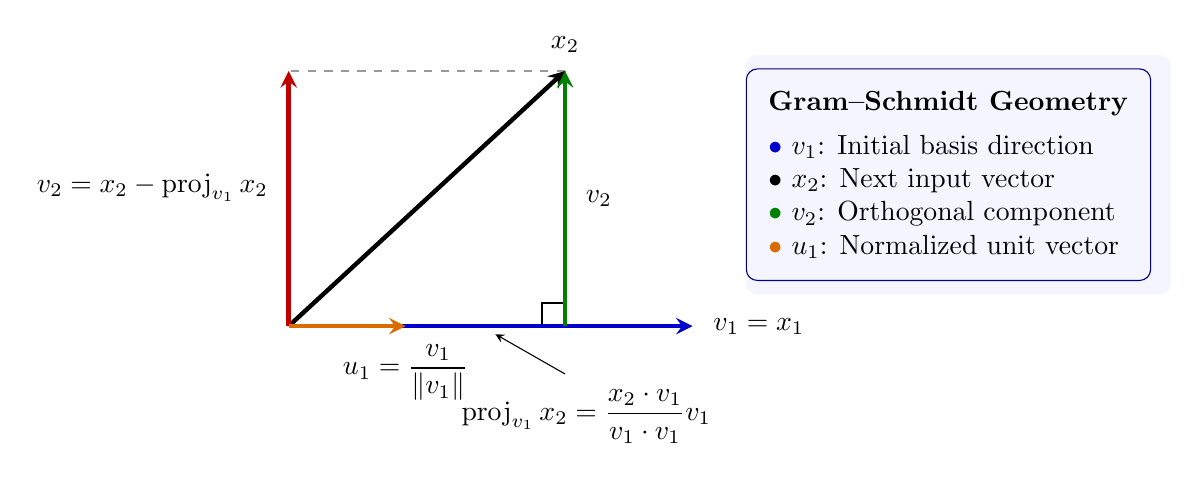
\begin{tikzpicture}[scale=1.35]
    % Layer 1: Fill backgrounds
    \fill[blue!4, rounded corners=4pt] (4.3, 0.3) rectangle (8.3, 2.55);

    % Layer 2: Grid lines, axes, projection dashed lines
    \draw[dashed, gray!80, thick] (2.6, 2.4) -- (2.6, 0);
    \draw[dashed, gray!80, thick] (2.6, 2.4) -- (0, 2.4);
    \draw[thick, black] (2.38, 0) -- (2.38, 0.22) -- (2.6, 0.22);

    % Layer 3: Primary plots and vectors
    \draw[->, >=stealth, ultra thick, blue!80!black] (0,0) -- (3.8,0);
    \draw[->, >=stealth, ultra thick, black] (0,0) -- (2.6,2.4);
    \draw[->, >=stealth, ultra thick, red!75!black] (0,0) -- (0,2.4);
    \draw[->, >=stealth, ultra thick, green!50!black] (2.6,0) -- (2.6,2.4);
    \draw[->, >=stealth, ultra thick, orange!85!black] (0,0) -- (1.1,0);

    % Callout arrow for projection vector on axis
    \draw[->, >=stealth, thin, black, shorten >=2pt] (2.6, -0.45) -- (1.9, -0.05);

    % Layer 4: Text nodes
    \node[black, right=4pt] at (3.8, 0) {$v_1 = x_1$};
    \node[black, above=3pt] at (2.6, 2.4) {$x_2$};
    \node[black, left=4pt] at (0, 1.3) {$\displaystyle v_2 = x_2 - \operatorname{proj}_{v_1} x_2$};
    \node[black, right=4pt] at (2.6, 1.2) {$v_2$};
    \node[black, below=3pt] at (1.1, 0) {$\displaystyle u_1 = \frac{v_1}{\|v_1\|}$};
    \node[black, below=2pt] at (2.8, -0.45) {$\displaystyle \operatorname{proj}_{v_1} x_2 = \frac{x_2 \cdot v_1}{v_1 \cdot v_1} v_1$};

    % Single-Node Multiline Legend
    \node[black, draw=blue!50!black, fill=blue!4, rounded corners=4pt, align=left, inner sep=8pt, anchor=west] at (4.3, 1.425) {%
        \textbf{Gram--Schmidt Geometry} \\[4pt]
        \textcolor{blue!80!black}{$\bullet$} $v_1$: Initial basis direction \\
        \textcolor{black}{$\bullet$} $x_2$: Next input vector \\
        \textcolor{green!50!black}{$\bullet$} $v_2$: Orthogonal component \\
        \textcolor{orange!85!black}{$\bullet$} $u_1$: Normalized unit vector%
    };
\end{tikzpicture}
\caption{Geometric intuition of the Gram--Schmidt orthogonalization step for two vectors.}
\end{figure}

\newpage

\section{Problem Sets}

\begin{enumerate}[label=\textbf{Problem \arabic*.}, leftmargin=*, itemsep=0.9em]

    \item The given set is a basis for a subspace $W \subset \mathbb{R}^3$. Use the Gram--Schmidt process to produce an orthogonal basis for $W$.
    \[
        x_1 = \begin{bmatrix} 1 \\ 2 \\ -2 \end{bmatrix}, \qquad x_2 = \begin{bmatrix} 4 \\ 2 \\ -5 \end{bmatrix}.
    \]

    \item Use the Gram--Schmidt process to produce an orthogonal basis with integer components for $W = \operatorname{Span}\{x_1, x_2\}$, where
    \[
        x_1 = \begin{bmatrix} 2 \\ 1 \\ -1 \end{bmatrix}, \qquad x_2 = \begin{bmatrix} 1 \\ 3 \\ 2 \end{bmatrix}.
    \]

    \item Use the Gram--Schmidt process to find an orthogonal basis for the subspace $W \subset \mathbb{R}^4$ spanned by
    \[
        x_1 = \begin{bmatrix} 1 \\ -1 \\ 1 \\ 1 \end{bmatrix}, \qquad x_2 = \begin{bmatrix} 3 \\ 1 \\ -1 \\ 3 \end{bmatrix}.
    \]

    \item Find an orthonormal basis for the subspace $W \subset \mathbb{R}^3$ spanned by
    \[
        x_1 = \begin{bmatrix} 3 \\ 4 \\ 0 \end{bmatrix}, \qquad x_2 = \begin{bmatrix} 2 \\ 11 \\ 12 \end{bmatrix}.
    \]

    \item Find an orthonormal basis for the subspace $W \subset \mathbb{R}^4$ spanned by
    \[
        x_1 = \begin{bmatrix} 1 \\ 1 \\ 0 \\ 1 \end{bmatrix}, \qquad x_2 = \begin{bmatrix} 2 \\ 0 \\ 1 \\ 1 \end{bmatrix}.
    \]

    \item Consider the plane $W = \{(x, y, z)^T \in \mathbb{R}^3 : x - 2y + z = 0\}$. Find a basis for $W$, and then apply the Gram--Schmidt process and normalization to produce an orthonormal basis for $W$.

    \item Apply the Gram--Schmidt process to find an orthogonal basis for $\mathbb{R}^3$ starting from the basis
    \[
        x_1 = \begin{bmatrix} 1 \\ 0 \\ 1 \end{bmatrix}, \qquad x_2 = \begin{bmatrix} 1 \\ 2 \\ 1 \end{bmatrix}, \qquad x_3 = \begin{bmatrix} 2 \\ 1 \\ 0 \end{bmatrix}.
    \]

    \item Find an orthogonal basis for the column space of the matrix
    \[
        A = \begin{bmatrix}
            1 & 2 & 5 \\
            1 & 0 & 1 \\
            1 & 2 & -1 \\
            1 & 0 & -1
        \end{bmatrix}.
    \]

    \item Find an orthogonal basis with integer entries for the column space of the matrix
    \[
        A = \begin{bmatrix}
            1 & 1 & 4 \\
            0 & 2 & 3 \\
            -1 & 1 & 1 \\
            1 & 1 & 0
        \end{bmatrix}.
    \]

    \item Find an orthogonal basis for the column space of the $5 \times 3$ matrix
    \[
        A = \begin{bmatrix}
            1 & 1 & 3 \\
            1 & 3 & 1 \\
            0 & 2 & 3 \\
            -1 & 1 & -1 \\
            1 & 1 & 3
        \end{bmatrix}.
    \]

    \item Apply the Gram--Schmidt process to construct an orthogonal basis for $\mathbb{R}^4$ from the basis
    \[
        x_1 = \begin{bmatrix} 1 \\ 1 \\ 1 \\ 1 \end{bmatrix}, \qquad
        x_2 = \begin{bmatrix} 2 \\ 0 \\ 0 \\ 2 \end{bmatrix}, \qquad
        x_3 = \begin{bmatrix} 2 \\ 2 \\ 0 \\ 0 \end{bmatrix}, \qquad
        x_4 = \begin{bmatrix} 0 \\ 3 \\ 1 \\ 0 \end{bmatrix}.
    \]

    \item The columns of $Q$ were obtained by applying the Gram--Schmidt process to the columns of $A$. Without re-running Gram--Schmidt, find the upper triangular matrix $R$ such that $A = QR$.
    \[
        A = \begin{bmatrix}
            2 & 4 \\
            2 & -2 \\
            2 & 4 \\
            2 & -2
        \end{bmatrix}, \qquad
        Q = \begin{bmatrix}
            1/2 & 1/2 \\
            1/2 & -1/2 \\
            1/2 & 1/2 \\
            1/2 & -1/2
        \end{bmatrix}.
    \]

    \item The columns of $Q$ were obtained by applying the Gram--Schmidt process to the columns of $A$. Find the upper triangular matrix $R$ such that $A = QR$, and verify explicitly that all entries below the main diagonal are zero.
    \[
        A = \begin{bmatrix}
            2 & 0 & -7 \\
            1 & 5 & 0 \\
            2 & 2 & -2 \\
            0 & 4 & 1
        \end{bmatrix}, \qquad
        Q = \begin{bmatrix}
            2/3 & -1/3 & -2/3 \\
            1/3 & 2/3 & 0 \\
            2/3 & 0 & 2/3 \\
            0 & 2/3 & -1/3
        \end{bmatrix}.
    \]

    \item Find a $QR$ factorization of the matrix
    \[
        A = \begin{bmatrix}
            1 & 4 \\
            2 & 2 \\
            2 & 5
        \end{bmatrix}.
    \]

    \item Find a $QR$ factorization of the $3 \times 3$ matrix
    \[
        A = \begin{bmatrix}
            1 & 2 & 1 \\
            1 & 0 & 5 \\
            0 & 2 & -1
        \end{bmatrix}.
    \]

    \item Find a $QR$ factorization of the $4 \times 3$ matrix
    \[
        A = \begin{bmatrix}
            1 & 1 & 0 \\
            1 & 3 & 4 \\
            1 & -1 & 2 \\
            1 & 1 & 2
        \end{bmatrix}.
    \]

    \item Find a $QR$ factorization of the $5 \times 3$ matrix
    \[
        A = \begin{bmatrix}
            1 & 3 & 4 \\
            1 & 1 & 0 \\
            -1 & -1 & 1 \\
            -1 & -3 & -3 \\
            1 & 2 & -1
        \end{bmatrix}.
    \]

    \item Find a $QR$ factorization of $A = \begin{bmatrix} 1 & 3 \\ 1 & -1 \\ 1 & 1 \\ 1 & 1 \end{bmatrix}$, and then use $Rx = Q^T b$ to solve the consistent linear system $Ax = b$ where $b = \begin{bmatrix} 5 \\ 1 \\ 3 \\ 3 \end{bmatrix}$ without computing $A^{-1}$ or $(A^T A)^{-1}$.

    \item Determine whether each statement is True or False, and give a rigorous justification:
    \begin{enumerate}[label=(\alph*)]
        \item If $\{v_1, v_2, v_3\}$ is an orthogonal basis for a subspace $W \subset \mathbb{R}^n$ and $c_1, c_2, c_3$ are nonzero scalars, then $\{c_1 v_1, c_2 v_2, c_3 v_3\}$ is also an orthogonal basis for $W$.
        \item If $\{v_1, v_2, v_3\}$ is an orthogonal set in a $3$-dimensional subspace $W \subset \mathbb{R}^n$, then $\{v_1, v_2, v_3\}$ must be a basis for $W$.
    \end{enumerate}

    \item Determine whether each statement is True or False, and give a rigorous justification:
    \begin{enumerate}[label=(\alph*)]
        \item If $A = QR$ where $Q \in \mathbb{R}^{m \times n}$ has orthonormal columns, then $Q Q^T = I_m$.
        \item If $A = QR$ is a $QR$ factorization of an $m \times n$ matrix $A$ with linearly independent columns, then every diagonal entry of $R$ must be nonzero.
    \end{enumerate}

    \item Suppose $A$ is an $m \times n$ matrix with linearly independent columns, and $A = QR$ where $Q \in \mathbb{R}^{m \times n}$ has orthonormal columns and $R \in \mathbb{R}^{n \times n}$ is upper triangular with strictly positive diagonal entries.
    \begin{enumerate}[label=(\alph*)]
        \item Prove that $R = Q^T A$ and that $R$ is invertible.
        \item Prove that such a $QR$ factorization is unique: if $A = Q_1 R_1 = Q_2 R_2$ where $Q_1, Q_2$ have orthonormal columns and $R_1, R_2$ are upper triangular with strictly positive diagonal entries, then $Q_1 = Q_2$ and $R_1 = R_2$.
    \end{enumerate}

    \item Let $\{x_1, \dots, x_p\}$ be a linearly independent set in $\mathbb{R}^n$, and define $\{v_1, \dots, v_p\}$ recursively by $v_1 = x_1$ and
    \[
        v_k = x_k - \sum_{j=1}^{k-1} \frac{x_k \cdot v_j}{v_j \cdot v_j} v_j \qquad (2 \le k \le p).
    \]
    Using mathematical induction on $k$, prove that for every $k \in \{1, \dots, p\}$:
    \begin{enumerate}[label=(\roman*)]
        \item $\{v_1, \dots, v_k\}$ is an orthogonal set of nonzero vectors, and
        \item $\operatorname{Span}\{v_1, \dots, v_k\} = \operatorname{Span}\{x_1, \dots, x_k\}$.
    \end{enumerate}

    \item In the polynomial inner product space $\mathbb{P}_2$ equipped with the inner product
    \[
        \langle f, g \rangle = \int_0^1 f(x) g(x)\,dx,
    \]
    apply the Gram--Schmidt process to the standard basis $\{1, x, x^2\}$ to find an orthogonal basis $\{v_1(x), v_2(x), v_3(x)\}$ of monic polynomials (the shifted Legendre polynomials).

    \item In the polynomial inner product space $\mathbb{P}_3$ equipped with $\langle f, g \rangle = \int_{-1}^1 f(x) g(x)\,dx$, given the first three orthogonal Legendre basis elements $v_1(x) = 1$, $v_2(x) = x$, and $v_3(x) = x^2 - \frac{1}{3}$, apply the next step of the Gram--Schmidt process to $x^3$ to find $v_4(x)$. Then normalize both $v_3(x)$ and $v_4(x)$.

    \item On $\mathbb{R}^3$, define the weighted inner product $\langle x, y \rangle_W = x_1 y_1 + 2 x_2 y_2 + 3 x_3 y_3$. Using $\langle \cdot, \cdot \rangle_W$, apply the Gram--Schmidt process to
    \[
        x_1 = \begin{bmatrix} 1 \\ 1 \\ 1 \end{bmatrix}, \qquad x_2 = \begin{bmatrix} 3 \\ 0 \\ 1 \end{bmatrix}
    \]
    to construct an orthogonal basis $\{v_1, v_2\}$ and an orthonormal basis $\{u_1, u_2\}$ with respect to $\langle \cdot, \cdot \rangle_W$.

    \item Apply the **Modified Gram--Schmidt (MGS)** algorithm step-by-step to the matrix
    \[
        A = \begin{bmatrix}
            1 & 3 & 2 \\
            1 & 1 & 0 \\
            0 & 2 & 2 \\
            0 & 0 & 2
        \end{bmatrix}
    \]
    to obtain its $QR$ factorization, explicitly displaying the intermediate updated columns $x_2^{(1)}$, $x_3^{(1)}$, and $x_3^{(2)}$ at each stage.

    \item In a machine learning linear regression problem $y = X\beta + \epsilon$, suppose the design matrix $X \in \mathbb{R}^{4 \times 2}$ and target vector $y \in \mathbb{R}^4$ are
    \[
        X = \begin{bmatrix}
            1 & 2 \\
            1 & 4 \\
            1 & 0 \\
            1 & 2
        \end{bmatrix}, \qquad
        y = \begin{bmatrix}
            3 \\
            7 \\
            1 \\
            5
        \end{bmatrix}.
    \]
    Compute the $QR$ factorization $X = QR$ and solve the Ordinary Least Squares (OLS) problem $\min_{\beta \in \mathbb{R}^2} \|y - X\beta\|_2^2$ via $R\beta = Q^T y$ and backward substitution (do not compute $(X^T X)^{-1}$).

    \item \textbf{(Find the Flaw)} Act as the grader for the following student solution. Identify the flaw, explain it in one sentence, and provide the corrected step and final orthogonal basis.
    
    \emph{Prompt:} Find an orthogonal basis for $W = \operatorname{Span}\{x_1, x_2, x_3\}$ where $x_1 = \begin{bmatrix} 1 \\ 1 \\ 0 \end{bmatrix}$, $x_2 = \begin{bmatrix} 1 \\ 0 \\ 1 \end{bmatrix}$, $x_3 = \begin{bmatrix} 0 \\ 2 \\ 2 \end{bmatrix}$.
    
    \emph{Student's Solution:}
    \begin{align*}
        v_1 &= x_1 = \begin{bmatrix} 1 \\ 1 \\ 0 \end{bmatrix}, \\
        v_2 &= x_2 - \frac{x_2 \cdot v_1}{v_1 \cdot v_1} v_1 = \begin{bmatrix} 1 \\ 0 \\ 1 \end{bmatrix} - \frac{1}{2}\begin{bmatrix} 1 \\ 1 \\ 0 \end{bmatrix} = \begin{bmatrix} 1/2 \\ -1/2 \\ 1 \end{bmatrix}, \\
        v_3 &= x_3 - \frac{x_3 \cdot v_1}{v_1 \cdot v_1} v_1 - \frac{x_3 \cdot x_2}{x_2 \cdot x_2} x_2 = \begin{bmatrix} 0 \\ 2 \\ 2 \end{bmatrix} - \frac{2}{2}\begin{bmatrix} 1 \\ 1 \\ 0 \end{bmatrix} - \frac{2}{2}\begin{bmatrix} 1 \\ 0 \\ 1 \end{bmatrix} = \begin{bmatrix} -2 \\ 1 \\ 1 \end{bmatrix}.
    \end{align*}

    \item \textbf{(Find the Flaw)} Act as the grader for the following student solution. Identify the flaw, explain why it invalidates the factorization, and provide the corrected $Q$ and $R$.
    
    \emph{Prompt:} Find the $QR$ factorization of $A = \begin{bmatrix} 3 & 10 \\ 0 & 5 \\ 4 & 5 \end{bmatrix}$.
    
    \emph{Student's Solution:}
    \begin{align*}
        v_1 &= \begin{bmatrix} 3 \\ 0 \\ 4 \end{bmatrix}, \qquad
        v_2 = \begin{bmatrix} 10 \\ 5 \\ 5 \end{bmatrix} - \frac{50}{25}\begin{bmatrix} 3 \\ 0 \\ 4 \end{bmatrix} = \begin{bmatrix} 4 \\ 5 \\ -3 \end{bmatrix}, \\
        Q &= \begin{bmatrix} 3 & 4 \\ 0 & 5 \\ 4 & -3 \end{bmatrix}, \qquad
        R = Q^T A = \begin{bmatrix} 3 & 0 & 4 \\ 4 & 5 & -3 \end{bmatrix} \begin{bmatrix} 3 & 10 \\ 0 & 5 \\ 4 & 5 \end{bmatrix} = \begin{bmatrix} 25 & 50 \\ 0 & 50 \end{bmatrix}.
    \end{align*}

    \item \textbf{(Find the Flaw)} Act as the grader for the following student solution. Identify the flaw, explain why it occurs, and provide the corrected matrix $R$.
    
    \emph{Prompt:} Find the $QR$ factorization of $A = \begin{bmatrix} 2 & 1 \\ 2 & 3 \\ 0 & 2 \end{bmatrix}$.
    
    \emph{Student's Solution:} ``Set $v_1 = [2, 2, 0]^T$ and scale it to $v_1' = [1, 1, 0]^T$. Then $v_2 = x_2 - \frac{x_2 \cdot v_1'}{v_1' \cdot v_1'} v_1' = [1, 3, 2]^T - \frac{4}{2}[1, 1, 0]^T = [-1, 1, 2]^T$. Normalizing gives $u_1 = \frac{1}{\sqrt{2}}[1, 1, 0]^T$ and $u_2 = \frac{1}{\sqrt{6}}[-1, 1, 2]^T$, so $Q = \begin{bmatrix} 1/\sqrt{2} & -1/\sqrt{6} \\ 1/\sqrt{2} & 1/\sqrt{6} \\ 0 & 2/\sqrt{6} \end{bmatrix}$. Reading the Gram--Schmidt coefficients directly gives $R = \begin{bmatrix} 1 & 2 \\ 0 & 1 \end{bmatrix}$.''

\end{enumerate}

\newpage

\section{Detailed Solutions}

\subsection{Solutions to Type 1: Gram--Schmidt for 2 Vectors (Problems 1--3)}

\textbf{Problem 1:} The given set is a basis for a subspace $W \subset \mathbb{R}^3$. Use the Gram--Schmidt process to produce an orthogonal basis for $W$.
\[
    x_1 = \begin{bmatrix} 1 \\ 2 \\ -2 \end{bmatrix}, \qquad x_2 = \begin{bmatrix} 4 \\ 2 \\ -5 \end{bmatrix}.
\]
\textbf{Solution:}
\begin{enumerate}[label=\textbf{Step \arabic*:}]
    \item Set $v_1 = x_1 = \begin{bmatrix} 1 \\ 2 \\ -2 \end{bmatrix}$. Compute $v_1 \cdot v_1$:
    \[
        v_1 \cdot v_1 = 1^2 + 2^2 + (-2)^2 = 1 + 4 + 4 = 9.
    \]
    \item Compute $v_2 = x_2 - \frac{x_2 \cdot v_1}{v_1 \cdot v_1} v_1$. First find $x_2 \cdot v_1$:
    \[
        x_2 \cdot v_1 = (4)(1) + (2)(2) + (-5)(-2) = 4 + 4 + 10 = 18.
    \]
    Substitute into the projection formula:
    \[
        v_2 = \begin{bmatrix} 4 \\ 2 \\ -5 \end{bmatrix} - \frac{18}{9}\begin{bmatrix} 1 \\ 2 \\ -2 \end{bmatrix}
        = \begin{bmatrix} 4 \\ 2 \\ -5 \end{bmatrix} - 2\begin{bmatrix} 1 \\ 2 \\ -2 \end{bmatrix}
        = \begin{bmatrix} 4 - 2 \\ 2 - 4 \\ -5 + 4 \end{bmatrix}
        = \begin{bmatrix} 2 \\ -2 \\ -1 \end{bmatrix}.
    \]
    \item Verify orthogonality: $v_1 \cdot v_2 = (1)(2) + (2)(-2) + (-2)(-1) = 2 - 4 + 2 = 0$.
\end{enumerate}
\textbf{Final Answer:} An orthogonal basis for $W$ is $\left\{ \begin{bmatrix} 1 \\ 2 \\ -2 \end{bmatrix}, \begin{bmatrix} 2 \\ -2 \\ -1 \end{bmatrix} \right\}$.

\vspace{0.8em}

\textbf{Problem 2:} Use the Gram--Schmidt process to produce an orthogonal basis with integer components for $W = \operatorname{Span}\{x_1, x_2\}$, where
\[
    x_1 = \begin{bmatrix} 2 \\ 1 \\ -1 \end{bmatrix}, \qquad x_2 = \begin{bmatrix} 1 \\ 3 \\ 2 \end{bmatrix}.
\]
\textbf{Solution:}
\begin{enumerate}[label=\textbf{Step \arabic*:}]
    \item Set $v_1 = x_1 = \begin{bmatrix} 2 \\ 1 \\ -1 \end{bmatrix}$. Compute $v_1 \cdot v_1 = 2^2 + 1^2 + (-1)^2 = 6$.
    \item Compute $x_2 \cdot v_1 = (1)(2) + (3)(1) + (2)(-1) = 2 + 3 - 2 = 3$. Then:
    \[
        v_2 = \begin{bmatrix} 1 \\ 3 \\ 2 \end{bmatrix} - \frac{3}{6}\begin{bmatrix} 2 \\ 1 \\ -1 \end{bmatrix}
        = \begin{bmatrix} 1 \\ 3 \\ 2 \end{bmatrix} - \frac{1}{2}\begin{bmatrix} 2 \\ 1 \\ -1 \end{bmatrix}
        = \begin{bmatrix} 0 \\ 5/2 \\ 5/2 \end{bmatrix}.
    \]
    \item Apply the scaling trick: multiply $v_2$ by $2$ to clear the denominator, giving $\begin{bmatrix} 0 \\ 5 \\ 5 \end{bmatrix}$, and divide by $5$ for the simplest integer form:
    \[
        v_2' = \frac{2}{5} v_2 = \begin{bmatrix} 0 \\ 1 \\ 1 \end{bmatrix}.
    \]
    Check orthogonality: $v_1 \cdot v_2' = (2)(0) + (1)(1) + (-1)(1) = 0$.
\end{enumerate}
\textbf{Final Answer:} An orthogonal basis with integer entries is $\left\{ \begin{bmatrix} 2 \\ 1 \\ -1 \end{bmatrix}, \begin{bmatrix} 0 \\ 1 \\ 1 \end{bmatrix} \right\}$.

\vspace{0.8em}

\textbf{Problem 3:} Use the Gram--Schmidt process to find an orthogonal basis for the subspace $W \subset \mathbb{R}^4$ spanned by
\[
    x_1 = \begin{bmatrix} 1 \\ -1 \\ 1 \\ 1 \end{bmatrix}, \qquad x_2 = \begin{bmatrix} 3 \\ 1 \\ -1 \\ 3 \end{bmatrix}.
\]
\textbf{Solution:}
\begin{enumerate}[label=\textbf{Step \arabic*:}]
    \item Set $v_1 = x_1 = \begin{bmatrix} 1 \\ -1 \\ 1 \\ 1 \end{bmatrix}$. Then $v_1 \cdot v_1 = 1^2 + (-1)^2 + 1^2 + 1^2 = 4$.
    \item Compute $x_2 \cdot v_1 = (3)(1) + (1)(-1) + (-1)(1) + (3)(1) = 3 - 1 - 1 + 3 = 4$. Thus:
    \[
        v_2 = \begin{bmatrix} 3 \\ 1 \\ -1 \\ 3 \end{bmatrix} - \frac{4}{4}\begin{bmatrix} 1 \\ -1 \\ 1 \\ 1 \end{bmatrix}
        = \begin{bmatrix} 2 \\ 2 \\ -2 \\ 2 \end{bmatrix}.
    \]
    Scaling by $\frac{1}{2}$ gives $v_2' = \begin{bmatrix} 1 \\ 1 \\ -1 \\ 1 \end{bmatrix}$. Check: $v_1 \cdot v_2' = 1 - 1 - 1 + 1 = 0$.
\end{enumerate}
\textbf{Final Answer:} An orthogonal basis for $W$ is $\left\{ \begin{bmatrix} 1 \\ -1 \\ 1 \\ 1 \end{bmatrix}, \begin{bmatrix} 1 \\ 1 \\ -1 \\ 1 \end{bmatrix} \right\}$ (or with $\begin{bmatrix} 2 \\ 2 \\ -2 \\ 2 \end{bmatrix}$).

\subsection{Solutions to Type 2: Orthonormal Basis Construction (Problems 4--6)}

\textbf{Problem 4:} Find an orthonormal basis for the subspace $W \subset \mathbb{R}^3$ spanned by
\[
    x_1 = \begin{bmatrix} 3 \\ 4 \\ 0 \end{bmatrix}, \qquad x_2 = \begin{bmatrix} 2 \\ 11 \\ 12 \end{bmatrix}.
\]
\textbf{Solution:}
\begin{enumerate}[label=\textbf{Step \arabic*:}]
    \item Set $v_1 = x_1 = \begin{bmatrix} 3 \\ 4 \\ 0 \end{bmatrix}$, so $v_1 \cdot v_1 = 3^2 + 4^2 + 0^2 = 25$.
    \item Compute $x_2 \cdot v_1 = (2)(3) + (11)(4) + (12)(0) = 6 + 44 = 50$. Then:
    \[
        v_2 = \begin{bmatrix} 2 \\ 11 \\ 12 \end{bmatrix} - \frac{50}{25}\begin{bmatrix} 3 \\ 4 \\ 0 \end{bmatrix}
        = \begin{bmatrix} 2 \\ 11 \\ 12 \end{bmatrix} - \begin{bmatrix} 6 \\ 8 \\ 0 \end{bmatrix}
        = \begin{bmatrix} -4 \\ 3 \\ 12 \end{bmatrix}.
    \]
    Check orthogonality: $v_1 \cdot v_2 = -12 + 12 + 0 = 0$.
    \item Normalize $v_1$ and $v_2$:
    \begin{align*}
        \|v_1\| &= \sqrt{25} = 5 \implies u_1 = \frac{1}{5}\begin{bmatrix} 3 \\ 4 \\ 0 \end{bmatrix} = \begin{bmatrix} 3/5 \\ 4/5 \\ 0 \end{bmatrix}, \\
        \|v_2\| &= \sqrt{(-4)^2 + 3^2 + 12^2} = \sqrt{16 + 9 + 144} = \sqrt{169} = 13 \implies u_2 = \frac{1}{13}\begin{bmatrix} -4 \\ 3 \\ 12 \end{bmatrix} = \begin{bmatrix} -4/13 \\ 3/13 \\ 12/13 \end{bmatrix}.
    \end{align*}
\end{enumerate}
\textbf{Final Answer:} The orthonormal basis is $\left\{ \begin{bmatrix} 3/5 \\ 4/5 \\ 0 \end{bmatrix}, \begin{bmatrix} -4/13 \\ 3/13 \\ 12/13 \end{bmatrix} \right\}$.

\vspace{0.8em}

\textbf{Problem 5:} Find an orthonormal basis for the subspace $W \subset \mathbb{R}^4$ spanned by
\[
    x_1 = \begin{bmatrix} 1 \\ 1 \\ 0 \\ 1 \end{bmatrix}, \qquad x_2 = \begin{bmatrix} 2 \\ 0 \\ 1 \\ 1 \end{bmatrix}.
\]
\textbf{Solution:}
\begin{enumerate}[label=\textbf{Step \arabic*:}]
    \item Set $v_1 = x_1 = \begin{bmatrix} 1 \\ 1 \\ 0 \\ 1 \end{bmatrix}$, with $v_1 \cdot v_1 = 1 + 1 + 0 + 1 = 3$.
    \item Compute $x_2 \cdot v_1 = 2 + 0 + 0 + 1 = 3$, so
    \[
        v_2 = \begin{bmatrix} 2 \\ 0 \\ 1 \\ 1 \end{bmatrix} - \frac{3}{3}\begin{bmatrix} 1 \\ 1 \\ 0 \\ 1 \end{bmatrix} = \begin{bmatrix} 1 \\ -1 \\ 1 \\ 0 \end{bmatrix}.
    \]
    Check: $v_1 \cdot v_2 = 1 - 1 + 0 + 0 = 0$.
    \item Normalize both vectors: $\|v_1\| = \sqrt{3}$ and $\|v_2\| = \sqrt{1 + 1 + 1 + 0} = \sqrt{3}$. Hence
    \[
        u_1 = \frac{1}{\sqrt{3}}\begin{bmatrix} 1 \\ 1 \\ 0 \\ 1 \end{bmatrix}, \qquad u_2 = \frac{1}{\sqrt{3}}\begin{bmatrix} 1 \\ -1 \\ 1 \\ 0 \end{bmatrix}.
    \]
\end{enumerate}
\textbf{Final Answer:} An orthonormal basis for $W$ is $\left\{ \begin{bmatrix} 1/\sqrt{3} \\ 1/\sqrt{3} \\ 0 \\ 1/\sqrt{3} \end{bmatrix}, \begin{bmatrix} 1/\sqrt{3} \\ -1/\sqrt{3} \\ 1/\sqrt{3} \\ 0 \end{bmatrix} \right\}$.

\vspace{0.8em}

\textbf{Problem 6:} Consider the plane $W = \{(x, y, z)^T \in \mathbb{R}^3 : x - 2y + z = 0\}$. Find a basis for $W$, and then apply the Gram--Schmidt process and normalization to produce an orthonormal basis for $W$.

\textbf{Solution:}
\begin{enumerate}[label=\textbf{Step \arabic*:}]
    \item Solve $x - 2y + z = 0$ for $x = 2y - z$ with free parameters $y = s$ and $z = t$:
    \[
        \begin{bmatrix} x \\ y \\ z \end{bmatrix} = \begin{bmatrix} 2s - t \\ s \\ t \end{bmatrix} = s\begin{bmatrix} 2 \\ 1 \\ 0 \end{bmatrix} + t\begin{bmatrix} -1 \\ 0 \\ 1 \end{bmatrix}.
    \]
    Thus $x_1 = \begin{bmatrix} 2 \\ 1 \\ 0 \end{bmatrix}$ and $x_2 = \begin{bmatrix} -1 \\ 0 \\ 1 \end{bmatrix}$ form a basis for $W$.
    \item Set $v_1 = x_1 = \begin{bmatrix} 2 \\ 1 \\ 0 \end{bmatrix}$, so $v_1 \cdot v_1 = 4 + 1 + 0 = 5$. Compute $x_2 \cdot v_1 = -2$:
    \[
        v_2 = \begin{bmatrix} -1 \\ 0 \\ 1 \end{bmatrix} - \frac{-2}{5}\begin{bmatrix} 2 \\ 1 \\ 0 \end{bmatrix} = \begin{bmatrix} -1/5 \\ 2/5 \\ 1 \end{bmatrix}.
    \]
    Multiply by $5$ to clear fractions: $v_2' = \begin{bmatrix} -1 \\ 2 \\ 5 \end{bmatrix}$. Check: $v_1 \cdot v_2' = -2 + 2 + 0 = 0$.
    \item Normalize: $\|v_1\| = \sqrt{5}$ and $\|v_2'\| = \sqrt{(-1)^2 + 2^2 + 5^2} = \sqrt{30}$, yielding
    \[
        u_1 = \frac{1}{\sqrt{5}}\begin{bmatrix} 2 \\ 1 \\ 0 \end{bmatrix}, \qquad u_2 = \frac{1}{\sqrt{30}}\begin{bmatrix} -1 \\ 2 \\ 5 \end{bmatrix}.
    \]
\end{enumerate}
\textbf{Final Answer:} An orthonormal basis for $W$ is $\left\{ \begin{bmatrix} 2/\sqrt{5} \\ 1/\sqrt{5} \\ 0 \end{bmatrix}, \begin{bmatrix} -1/\sqrt{30} \\ 2/\sqrt{30} \\ 5/\sqrt{30} \end{bmatrix} \right\}$.

\subsection{Solutions to Type 3: Gram--Schmidt for 3 or 4 Vectors in Higher Dimensions (Problems 7--11)}

\textbf{Problem 7:} Apply the Gram--Schmidt process to find an orthogonal basis for $\mathbb{R}^3$ starting from the basis
\[
    x_1 = \begin{bmatrix} 1 \\ 0 \\ 1 \end{bmatrix}, \qquad x_2 = \begin{bmatrix} 1 \\ 2 \\ 1 \end{bmatrix}, \qquad x_3 = \begin{bmatrix} 2 \\ 1 \\ 0 \end{bmatrix}.
\]
\textbf{Solution:}
\begin{enumerate}[label=\textbf{Step \arabic*:}]
    \item Set $v_1 = x_1 = \begin{bmatrix} 1 \\ 0 \\ 1 \end{bmatrix}$, with $v_1 \cdot v_1 = 2$.
    \item Compute $x_2 \cdot v_1 = 1 + 0 + 1 = 2$:
    \[
        v_2 = \begin{bmatrix} 1 \\ 2 \\ 1 \end{bmatrix} - \frac{2}{2}\begin{bmatrix} 1 \\ 0 \\ 1 \end{bmatrix} = \begin{bmatrix} 0 \\ 2 \\ 0 \end{bmatrix}.
    \]
    Scale by $\frac{1}{2}$: $v_2' = \begin{bmatrix} 0 \\ 1 \\ 0 \end{bmatrix}$, with $v_2' \cdot v_2' = 1$.
    \item Compute $x_3 \cdot v_1 = 2 + 0 + 0 = 2$ and $x_3 \cdot v_2' = 0 + 1 + 0 = 1$:
    \[
        v_3 = \begin{bmatrix} 2 \\ 1 \\ 0 \end{bmatrix} - \frac{2}{2}\begin{bmatrix} 1 \\ 0 \\ 1 \end{bmatrix} - \frac{1}{1}\begin{bmatrix} 0 \\ 1 \\ 0 \end{bmatrix} = \begin{bmatrix} 1 \\ 0 \\ -1 \end{bmatrix}.
    \]
    Check: $v_1 \cdot v_2' = 0$, $v_1 \cdot v_3 = 0$, and $v_2' \cdot v_3 = 0$.
\end{enumerate}
\textbf{Final Answer:} An orthogonal basis for $\mathbb{R}^3$ is $\left\{ \begin{bmatrix} 1 \\ 0 \\ 1 \end{bmatrix}, \begin{bmatrix} 0 \\ 1 \\ 0 \end{bmatrix}, \begin{bmatrix} 1 \\ 0 \\ -1 \end{bmatrix} \right\}$.

\vspace{0.8em}

\textbf{Problem 8:} Find an orthogonal basis for the column space of the matrix
\[
    A = \begin{bmatrix}
        1 & 2 & 5 \\
        1 & 0 & 1 \\
        1 & 2 & -1 \\
        1 & 0 & -1
    \end{bmatrix}.
\]
\textbf{Solution:} Denote the columns of $A$ by $x_1, x_2, x_3$.
\begin{enumerate}[label=\textbf{Step \arabic*:}]
    \item Set $v_1 = x_1 = \begin{bmatrix} 1 \\ 1 \\ 1 \\ 1 \end{bmatrix}$, so $v_1 \cdot v_1 = 4$.
    \item Compute $x_2 \cdot v_1 = 2 + 0 + 2 + 0 = 4$:
    \[
        v_2 = \begin{bmatrix} 2 \\ 0 \\ 2 \\ 0 \end{bmatrix} - \frac{4}{4}\begin{bmatrix} 1 \\ 1 \\ 1 \\ 1 \end{bmatrix} = \begin{bmatrix} 1 \\ -1 \\ 1 \\ -1 \end{bmatrix}.
    \]
    Then $v_2 \cdot v_2 = 4$ and $v_1 \cdot v_2 = 1 - 1 + 1 - 1 = 0$.
    \item Compute $x_3 \cdot v_1 = 5 + 1 - 1 - 1 = 4$ and $x_3 \cdot v_2 = 5 - 1 - 1 + 1 = 4$:
    \[
        v_3 = \begin{bmatrix} 5 \\ 1 \\ -1 \\ -1 \end{bmatrix} - \frac{4}{4}\begin{bmatrix} 1 \\ 1 \\ 1 \\ 1 \end{bmatrix} - \frac{4}{4}\begin{bmatrix} 1 \\ -1 \\ 1 \\ -1 \end{bmatrix}
        = \begin{bmatrix} 5 - 1 - 1 \\ 1 - 1 + 1 \\ -1 - 1 - 1 \\ -1 - 1 + 1 \end{bmatrix}
        = \begin{bmatrix} 3 \\ 1 \\ -3 \\ -1 \end{bmatrix}.
    \]
    Check: $v_1 \cdot v_3 = 3 + 1 - 3 - 1 = 0$ and $v_2 \cdot v_3 = 3 - 1 - 3 + 1 = 0$.
\end{enumerate}
\textbf{Final Answer:} An orthogonal basis for $\operatorname{Col}(A)$ is $\left\{ \begin{bmatrix} 1 \\ 1 \\ 1 \\ 1 \end{bmatrix}, \begin{bmatrix} 1 \\ -1 \\ 1 \\ -1 \end{bmatrix}, \begin{bmatrix} 3 \\ 1 \\ -3 \\ -1 \end{bmatrix} \right\}$.

\vspace{0.8em}

\textbf{Problem 9:} Find an orthogonal basis with integer entries for the column space of the matrix
\[
    A = \begin{bmatrix}
        1 & 1 & 4 \\
        0 & 2 & 3 \\
        -1 & 1 & 1 \\
        1 & 1 & 0
    \end{bmatrix}.
\]
\textbf{Solution:} Let $x_1, x_2, x_3$ be the columns of $A$.
\begin{enumerate}[label=\textbf{Step \arabic*:}]
    \item Set $v_1 = x_1 = \begin{bmatrix} 1 \\ 0 \\ -1 \\ 1 \end{bmatrix}$, so $v_1 \cdot v_1 = 3$.
    \item Compute $x_2 \cdot v_1 = 1 + 0 - 1 + 1 = 1$:
    \[
        v_2 = \begin{bmatrix} 1 \\ 2 \\ 1 \\ 1 \end{bmatrix} - \frac{1}{3}\begin{bmatrix} 1 \\ 0 \\ -1 \\ 1 \end{bmatrix} = \begin{bmatrix} 2/3 \\ 2 \\ 4/3 \\ 2/3 \end{bmatrix}.
    \]
    Multiply by $\frac{3}{2}$ to obtain the simplest integer vector:
    \[
        v_2' = \begin{bmatrix} 1 \\ 3 \\ 2 \\ 1 \end{bmatrix}, \qquad v_2' \cdot v_2' = 1 + 9 + 4 + 1 = 15.
    \]
    Check: $v_1 \cdot v_2' = 1 + 0 - 2 + 1 = 0$.
    \item Compute $x_3 \cdot v_1 = 4 + 0 - 1 + 0 = 3$ and $x_3 \cdot v_2' = 4 + 6 + 2 + 0$? Wait: check carefully!
    \[
        x_3 \cdot v_2' = (4)(1) + (3)(3) + (1)(2) + (0)(1) = 4 + 9 + 2 + 0 = 15.
    \]
    Substitute into the Gram--Schmidt formula:
    \[
        v_3 = \begin{bmatrix} 4 \\ 3 \\ 1 \\ 0 \end{bmatrix} - \frac{3}{3}\begin{bmatrix} 1 \\ 0 \\ -1 \\ 1 \end{bmatrix} - \frac{15}{15}\begin{bmatrix} 1 \\ 3 \\ 2 \\ 1 \end{bmatrix}
        = \begin{bmatrix} 4 - 1 - 1 \\ 3 - 0 - 3 \\ 1 + 1 - 2 \\ 0 - 1 - 1 \end{bmatrix}
        = \begin{bmatrix} 2 \\ 0 \\ 0 \\ -2 \end{bmatrix}.
    \]
    Scale by $\frac{1}{2}$: $v_3' = \begin{bmatrix} 1 \\ 0 \\ 0 \\ -1 \end{bmatrix}$. Check: $v_1 \cdot v_3' = 1 - 1 = 0$ and $v_2' \cdot v_3' = 1 - 1 = 0$.
\end{enumerate}
\textbf{Final Answer:} An orthogonal basis for $\operatorname{Col}(A)$ is $\left\{ \begin{bmatrix} 1 \\ 0 \\ -1 \\ 1 \end{bmatrix}, \begin{bmatrix} 1 \\ 3 \\ 2 \\ 1 \end{bmatrix}, \begin{bmatrix} 1 \\ 0 \\ 0 \\ -1 \end{bmatrix} \right\}$.

\vspace{0.8em}

\textbf{Problem 10:} Find an orthogonal basis for the column space of the $5 \times 3$ matrix
\[
    A = \begin{bmatrix}
        1 & 1 & 3 \\
        1 & 3 & 1 \\
        0 & 2 & 3 \\
        -1 & 1 & -1 \\
        1 & 1 & 3
    \end{bmatrix}.
\]
\textbf{Solution:} Let $x_1, x_2, x_3$ be the columns of $A$.
\begin{enumerate}[label=\textbf{Step \arabic*:}]
    \item Set $v_1 = x_1 = \begin{bmatrix} 1 \\ 1 \\ 0 \\ -1 \\ 1 \end{bmatrix}$, with $v_1 \cdot v_1 = 1 + 1 + 0 + 1 + 1 = 4$.
    \item Compute $x_2 \cdot v_1 = 1 + 3 + 0 - 1 + 1 = 4$:
    \[
        v_2 = \begin{bmatrix} 1 \\ 3 \\ 2 \\ 1 \\ 1 \end{bmatrix} - \frac{4}{4}\begin{bmatrix} 1 \\ 1 \\ 0 \\ -1 \\ 1 \end{bmatrix} = \begin{bmatrix} 0 \\ 2 \\ 2 \\ 2 \\ 0 \end{bmatrix}.
    \]
    Scale by $\frac{1}{2}$: $v_2' = \begin{bmatrix} 0 \\ 1 \\ 1 \\ 1 \\ 0 \end{bmatrix}$, with $v_2' \cdot v_2' = 3$. Check: $v_1 \cdot v_2' = 0 + 1 + 0 - 1 + 0 = 0$.
    \item Compute $x_3 \cdot v_1 = 3 + 1 + 0 + 1 + 3 = 8$ and $x_3 \cdot v_2' = 0 + 1 + 3 - 1 + 0 = 3$:
    \[
        v_3 = \begin{bmatrix} 3 \\ 1 \\ 3 \\ -1 \\ 3 \end{bmatrix} - \frac{8}{4}\begin{bmatrix} 1 \\ 1 \\ 0 \\ -1 \\ 1 \end{bmatrix} - \frac{3}{3}\begin{bmatrix} 0 \\ 1 \\ 1 \\ 1 \\ 0 \end{bmatrix}
        = \begin{bmatrix} 3 - 2 - 0 \\ 1 - 2 - 1 \\ 3 - 0 - 1 \\ -1 + 2 - 1 \\ 3 - 2 - 0 \end{bmatrix}
        = \begin{bmatrix} 1 \\ -2 \\ 2 \\ 0 \\ 1 \end{bmatrix}.
    \]
    Check: $v_1 \cdot v_3 = 1 - 2 + 0 + 0 + 1 = 0$ and $v_2' \cdot v_3 = 0 - 2 + 2 + 0 + 0 = 0$.
\end{enumerate}
\textbf{Final Answer:} An orthogonal basis for $\operatorname{Col}(A)$ is $\left\{ \begin{bmatrix} 1 \\ 1 \\ 0 \\ -1 \\ 1 \end{bmatrix}, \begin{bmatrix} 0 \\ 1 \\ 1 \\ 1 \\ 0 \end{bmatrix}, \begin{bmatrix} 1 \\ -2 \\ 2 \\ 0 \\ 1 \end{bmatrix} \right\}$.

\vspace{0.8em}

\textbf{Problem 11:} Apply the Gram--Schmidt process to construct an orthogonal basis for $\mathbb{R}^4$ from the basis
\[
    x_1 = \begin{bmatrix} 1 \\ 1 \\ 1 \\ 1 \end{bmatrix}, \qquad
    x_2 = \begin{bmatrix} 2 \\ 0 \\ 0 \\ 2 \end{bmatrix}, \qquad
    x_3 = \begin{bmatrix} 2 \\ 2 \\ 0 \\ 0 \end{bmatrix}, \qquad
    x_4 = \begin{bmatrix} 0 \\ 3 \\ 1 \\ 0 \end{bmatrix}.
\]
\textbf{Solution:}
\begin{enumerate}[label=\textbf{Step \arabic*:}]
    \item Set $v_1 = x_1 = \begin{bmatrix} 1 \\ 1 \\ 1 \\ 1 \end{bmatrix}$, with $v_1 \cdot v_1 = 4$.
    \item $x_2 \cdot v_1 = 2 + 0 + 0 + 2 = 4$, so
    \[
        v_2 = \begin{bmatrix} 2 \\ 0 \\ 0 \\ 2 \end{bmatrix} - \frac{4}{4}\begin{bmatrix} 1 \\ 1 \\ 1 \\ 1 \end{bmatrix} = \begin{bmatrix} 1 \\ -1 \\ -1 \\ 1 \end{bmatrix}, \qquad v_2 \cdot v_2 = 4.
    \]
    \item $x_3 \cdot v_1 = 2 + 2 + 0 + 0 = 4$ and $x_3 \cdot v_2 = 2 - 2 + 0 + 0 = 0$, so
    \[
        v_3 = \begin{bmatrix} 2 \\ 2 \\ 0 \\ 0 \end{bmatrix} - \frac{4}{4}\begin{bmatrix} 1 \\ 1 \\ 1 \\ 1 \end{bmatrix} - 0 = \begin{bmatrix} 1 \\ 1 \\ -1 \\ -1 \end{bmatrix}, \qquad v_3 \cdot v_3 = 4.
    \]
    \item Compute $x_4 \cdot v_1 = 0 + 3 + 1 + 0 = 4$, $x_4 \cdot v_2 = 0 - 3 - 1 + 0 = -4$, and $x_4 \cdot v_3 = 0 + 3 - 1 + 0 = 2$:
    \[
        v_4 = \begin{bmatrix} 0 \\ 3 \\ 1 \\ 0 \end{bmatrix} - \frac{4}{4}\begin{bmatrix} 1 \\ 1 \\ 1 \\ 1 \end{bmatrix} - \frac{-4}{4}\begin{bmatrix} 1 \\ -1 \\ -1 \\ 1 \end{bmatrix} - \frac{2}{4}\begin{bmatrix} 1 \\ 1 \\ -1 \\ -1 \end{bmatrix}
        = \begin{bmatrix} 0 - 1 + 1 - 1/2 \\ 3 - 1 - 1 - 1/2 \\ 1 - 1 - 1 + 1/2 \\ 0 - 1 + 1 + 1/2 \end{bmatrix}
        = \begin{bmatrix} -1/2 \\ 1/2 \\ -1/2 \\ 1/2 \end{bmatrix}.
    \]
    Scale by $2$: $v_4' = \begin{bmatrix} -1 \\ 1 \\ -1 \\ 1 \end{bmatrix}$. All six pairwise dot products vanish: $v_i \cdot v_j = 0$ for $i \neq j$.
\end{enumerate}
\textbf{Final Answer:} An orthogonal basis for $\mathbb{R}^4$ is $\left\{ \begin{bmatrix} 1 \\ 1 \\ 1 \\ 1 \end{bmatrix}, \begin{bmatrix} 1 \\ -1 \\ -1 \\ 1 \end{bmatrix}, \begin{bmatrix} 1 \\ 1 \\ -1 \\ -1 \end{bmatrix}, \begin{bmatrix} -1 \\ 1 \\ -1 \\ 1 \end{bmatrix} \right\}$.

\subsection{Solutions to Type 4a: Finding $R$ Given $A$ and $Q$ (Problems 12--13)}

\textbf{Problem 12:} The columns of $Q$ were obtained by applying the Gram--Schmidt process to the columns of $A$. Without re-running Gram--Schmidt, find the upper triangular matrix $R$ such that $A = QR$.
\[
    A = \begin{bmatrix}
        2 & 4 \\
        2 & -2 \\
        2 & 4 \\
        2 & -2
    \end{bmatrix}, \qquad
    Q = \begin{bmatrix}
        1/2 & 1/2 \\
        1/2 & -1/2 \\
        1/2 & 1/2 \\
        1/2 & -1/2
    \end{bmatrix}.
\]
\textbf{Solution:} Since $Q$ has orthonormal columns, $Q^T Q = I_2$. Left-multiplying $A = QR$ by $Q^T$ gives $R = Q^T A$:
\[
    R = \begin{bmatrix}
        1/2 & 1/2 & 1/2 & 1/2 \\
        1/2 & -1/2 & 1/2 & -1/2
    \end{bmatrix}
    \begin{bmatrix}
        2 & 4 \\
        2 & -2 \\
        2 & 4 \\
        2 & -2
    \end{bmatrix}.
\]
Compute each entry:
\begin{align*}
    r_{11} &= \frac{1}{2}(2 + 2 + 2 + 2) = 4, & r_{12} &= \frac{1}{2}(4 - 2 + 4 - 2) = 2, \\
    r_{21} &= \frac{1}{2}(2 - 2 + 2 - 2) = 0, & r_{22} &= \frac{1}{2}(4 + 2 + 4 + 2) = 6.
\end{align*}
\textbf{Final Answer:} $R = \begin{bmatrix} 4 & 2 \\ 0 & 6 \end{bmatrix}$.

\vspace{0.8em}

\textbf{Problem 13:} The columns of $Q$ were obtained by applying the Gram--Schmidt process to the columns of $A$. Find the upper triangular matrix $R$ such that $A = QR$, and verify explicitly that all entries below the main diagonal are zero.
\[
    A = \begin{bmatrix}
        2 & 0 & -7 \\
        1 & 5 & 0 \\
        2 & 2 & -2 \\
        0 & 4 & 1
    \end{bmatrix}, \qquad
    Q = \begin{bmatrix}
        2/3 & -1/3 & -2/3 \\
        1/3 & 2/3 & 0 \\
        2/3 & 0 & 2/3 \\
        0 & 2/3 & -1/3
    \end{bmatrix}.
\]
\textbf{Solution:} Compute $R = Q^T A$:
\[
    R = \frac{1}{3}
    \begin{bmatrix}
        2 & 1 & 2 & 0 \\
        -1 & 2 & 0 & 2 \\
        -2 & 0 & 2 & -1
    \end{bmatrix}
    \begin{bmatrix}
        2 & 0 & -7 \\
        1 & 5 & 0 \\
        2 & 2 & -2 \\
        0 & 4 & 1
    \end{bmatrix}.
\]
Evaluating all nine dot products:
\begin{align*}
    r_{11} &= \frac{1}{3}(4 + 1 + 4 + 0) = 3, & r_{12} &= \frac{1}{3}(0 + 5 + 4 + 0) = 3, & r_{13} &= \frac{1}{3}(-14 + 0 - 4 + 0) = -6, \\
    r_{21} &= \frac{1}{3}(-2 + 2 + 0 + 0) = 0, & r_{22} &= \frac{1}{3}(0 + 10 + 0 + 8) = 6, & r_{23} &= \frac{1}{3}(7 + 0 + 0 + 2) = 3, \\
    r_{31} &= \frac{1}{3}(-4 + 0 + 4 + 0) = 0, & r_{32} &= \frac{1}{3}(0 + 0 + 4 - 4) = 0, & r_{33} &= \frac{1}{3}(14 + 0 - 4 - 1) = 3.
\end{align*}
Indeed, $r_{21} = r_{31} = r_{32} = 0$, confirming upper triangularity.

\textbf{Final Answer:} $R = \begin{bmatrix} 3 & 3 & -6 \\ 0 & 6 & 3 \\ 0 & 0 & 3 \end{bmatrix}$.

\subsection{Solutions to Type 4b: Full $QR$ Factorization and Linear Systems (Problems 14--18)}

\textbf{Problem 14:} Find a $QR$ factorization of the matrix $A = \begin{bmatrix} 1 & 4 \\ 2 & 2 \\ 2 & 5 \end{bmatrix}$.

\textbf{Solution:}
\begin{enumerate}[label=\textbf{Step \arabic*:}]
    \item Let $x_1 = \begin{bmatrix} 1 \\ 2 \\ 2 \end{bmatrix}$ and $x_2 = \begin{bmatrix} 4 \\ 2 \\ 5 \end{bmatrix}$. Set $v_1 = x_1$, with $v_1 \cdot v_1 = 1 + 4 + 4 = 9$.
    \item Compute $x_2 \cdot v_1 = 4 + 4 + 10 = 18$, so
    \[
        v_2 = \begin{bmatrix} 4 \\ 2 \\ 5 \end{bmatrix} - \frac{18}{9}\begin{bmatrix} 1 \\ 2 \\ 2 \end{bmatrix} = \begin{bmatrix} 2 \\ -2 \\ 1 \end{bmatrix}.
    \]
    \item Normalize: $\|v_1\| = \sqrt{9} = 3$ and $\|v_2\| = \sqrt{4 + 4 + 1} = 3$, giving
    \[
        Q = \begin{bmatrix} 1/3 & 2/3 \\ 2/3 & -2/3 \\ 2/3 & 1/3 \end{bmatrix}.
    \]
    \item Compute $R = Q^T A$:
    \[
        R = \begin{bmatrix} 1/3 & 2/3 & 2/3 \\ 2/3 & -2/3 & 1/3 \end{bmatrix} \begin{bmatrix} 1 & 4 \\ 2 & 2 \\ 2 & 5 \end{bmatrix} = \begin{bmatrix} 3 & 6 \\ 0 & 3 \end{bmatrix}.
    \]
\end{enumerate}
\textbf{Final Answer:} $Q = \begin{bmatrix} 1/3 & 2/3 \\ 2/3 & -2/3 \\ 2/3 & 1/3 \end{bmatrix}$ and $R = \begin{bmatrix} 3 & 6 \\ 0 & 3 \end{bmatrix}$.

\vspace{0.8em}

\textbf{Problem 15:} Find a $QR$ factorization of the $3 \times 3$ matrix $A = \begin{bmatrix} 1 & 2 & 1 \\ 1 & 0 & 5 \\ 0 & 2 & -1 \end{bmatrix}$.

\textbf{Solution:}
\begin{enumerate}[label=\textbf{Step \arabic*:}]
    \item Set $v_1 = x_1 = \begin{bmatrix} 1 \\ 1 \\ 0 \end{bmatrix}$, so $v_1 \cdot v_1 = 2$ and $\|v_1\| = \sqrt{2}$.
    \item Compute $x_2 \cdot v_1 = 2 + 0 + 0 = 2$:
    \[
        v_2 = \begin{bmatrix} 2 \\ 0 \\ 2 \end{bmatrix} - \frac{2}{2}\begin{bmatrix} 1 \\ 1 \\ 0 \end{bmatrix} = \begin{bmatrix} 1 \\ -1 \\ 2 \end{bmatrix}, \qquad v_2 \cdot v_2 = 6, \quad \|v_2\| = \sqrt{6}.
    \]
    \item Compute $x_3 \cdot v_1 = 1 + 5 + 0 = 6$ and $x_3 \cdot v_2 = 1 - 5 - 2 = -6$:
    \[
        v_3 = \begin{bmatrix} 1 \\ 5 \\ -1 \end{bmatrix} - \frac{6}{2}\begin{bmatrix} 1 \\ 1 \\ 0 \end{bmatrix} - \frac{-6}{6}\begin{bmatrix} 1 \\ -1 \\ 2 \end{bmatrix}
        = \begin{bmatrix} 1 - 3 + 1 \\ 5 - 3 - 1 \\ -1 - 0 + 2 \end{bmatrix}
        = \begin{bmatrix} -1 \\ 1 \\ 1 \end{bmatrix}, \qquad \|v_3\| = \sqrt{3}.
    \]
    \item Normalize to form $Q$:
    \[
        Q = \begin{bmatrix}
            1/\sqrt{2} & 1/\sqrt{6} & -1/\sqrt{3} \\
            1/\sqrt{2} & -1/\sqrt{6} & 1/\sqrt{3} \\
            0 & 2/\sqrt{6} & 1/\sqrt{3}
        \end{bmatrix}.
    \]
    \item Compute $R = Q^T A$ via $r_{ij} = u_i \cdot x_j$ for $i \le j$:
    \begin{align*}
        r_{11} &= u_1 \cdot x_1 = \frac{2}{\sqrt{2}} = \sqrt{2}, & r_{12} &= u_1 \cdot x_2 = \frac{2}{\sqrt{2}} = \sqrt{2}, & r_{13} &= u_1 \cdot x_3 = \frac{6}{\sqrt{2}} = 3\sqrt{2}, \\
        r_{22} &= u_2 \cdot x_2 = \frac{6}{\sqrt{6}} = \sqrt{6}, & r_{23} &= u_2 \cdot x_3 = \frac{-6}{\sqrt{6}} = -\sqrt{6}, & r_{33} &= u_3 \cdot x_3 = \frac{3}{\sqrt{3}} = \sqrt{3}.
    \end{align*}
\end{enumerate}
\textbf{Final Answer:}
\[
    Q = \begin{bmatrix}
        1/\sqrt{2} & 1/\sqrt{6} & -1/\sqrt{3} \\
        1/\sqrt{2} & -1/\sqrt{6} & 1/\sqrt{3} \\
        0 & 2/\sqrt{6} & 1/\sqrt{3}
    \end{bmatrix}, \qquad
    R = \begin{bmatrix}
        \sqrt{2} & \sqrt{2} & 3\sqrt{2} \\
        0 & \sqrt{6} & -\sqrt{6} \\
        0 & 0 & \sqrt{3}
    \end{bmatrix}.
\]

\vspace{0.8em}

\textbf{Problem 16:} Find a $QR$ factorization of the $4 \times 3$ matrix $A = \begin{bmatrix} 1 & 1 & 0 \\ 1 & 3 & 4 \\ 1 & -1 & 2 \\ 1 & 1 & 2 \end{bmatrix}$.

\textbf{Solution:}
\begin{enumerate}[label=\textbf{Step \arabic*:}]
    \item Set $v_1 = x_1 = \begin{bmatrix} 1 \\ 1 \\ 1 \\ 1 \end{bmatrix}$, so $v_1 \cdot v_1 = 4$, $\|v_1\| = 2$, and $u_1 = \frac{1}{2}\begin{bmatrix} 1 \\ 1 \\ 1 \\ 1 \end{bmatrix}$.
    \item Compute $x_2 \cdot v_1 = 1 + 3 - 1 + 1 = 4$, so $v_2 = \begin{bmatrix} 1 \\ 3 \\ -1 \\ 1 \end{bmatrix} - \begin{bmatrix} 1 \\ 1 \\ 1 \\ 1 \end{bmatrix} = \begin{bmatrix} 0 \\ 2 \\ -2 \\ 0 \end{bmatrix}$. Scale by $\frac{1}{2}$ to get $v_2' = \begin{bmatrix} 0 \\ 1 \\ -1 \\ 0 \end{bmatrix}$, with $\|v_2'\| = \sqrt{2}$ and $u_2 = \frac{1}{\sqrt{2}}\begin{bmatrix} 0 \\ 1 \\ -1 \\ 0 \end{bmatrix}$.
    \item Compute $x_3 \cdot v_1 = 0 + 4 + 2 + 2 = 8$ and $x_3 \cdot v_2' = 0 + 4 - 2 + 0 = 2$:
    \[
        v_3 = \begin{bmatrix} 0 \\ 4 \\ 2 \\ 2 \end{bmatrix} - \frac{8}{4}\begin{bmatrix} 1 \\ 1 \\ 1 \\ 1 \end{bmatrix} - \frac{2}{2}\begin{bmatrix} 0 \\ 1 \\ -1 \\ 0 \end{bmatrix} = \begin{bmatrix} -2 \\ 1 \\ 1 \\ 0 \end{bmatrix}, \qquad \|v_3\| = \sqrt{6}, \quad u_3 = \frac{1}{\sqrt{6}}\begin{bmatrix} -2 \\ 1 \\ 1 \\ 0 \end{bmatrix}.
    \]
    \item Compute $R = Q^T A$ using $r_{ij} = u_i \cdot x_j$ for $i \le j$:
    \begin{align*}
        r_{11} &= \frac{4}{2} = 2, & r_{12} &= \frac{4}{2} = 2, & r_{13} &= \frac{8}{2} = 4, \\
        r_{22} &= \frac{4}{\sqrt{2}} = 2\sqrt{2}, & r_{23} &= \frac{2}{\sqrt{2}} = \sqrt{2}, & r_{33} &= \frac{6}{\sqrt{6}} = \sqrt{6}.
    \end{align*}
\end{enumerate}
\textbf{Final Answer:}
\[
    Q = \begin{bmatrix}
        1/2 & 0 & -2/\sqrt{6} \\
        1/2 & 1/\sqrt{2} & 1/\sqrt{6} \\
        1/2 & -1/\sqrt{2} & 1/\sqrt{6} \\
        1/2 & 0 & 0
    \end{bmatrix}, \qquad
    R = \begin{bmatrix}
        2 & 2 & 4 \\
        0 & 2\sqrt{2} & \sqrt{2} \\
        0 & 0 & \sqrt{6}
    \end{bmatrix}.
\]

\vspace{0.8em}

\textbf{Problem 17:} Find a $QR$ factorization of the $5 \times 3$ matrix
\[
    A = \begin{bmatrix}
        1 & 3 & 4 \\
        1 & 1 & 0 \\
        -1 & -1 & 1 \\
        -1 & -3 & -3 \\
        1 & 2 & -1
    \end{bmatrix}.
\]
\textbf{Solution:}
\begin{enumerate}[label=\textbf{Step \arabic*:}]
    \item Set $v_1 = x_1 = \begin{bmatrix} 1 \\ 1 \\ -1 \\ -1 \\ 1 \end{bmatrix}$, so $v_1 \cdot v_1 = 5$, $\|v_1\| = \sqrt{5}$, and $u_1 = \frac{1}{\sqrt{5}}\begin{bmatrix} 1 \\ 1 \\ -1 \\ -1 \\ 1 \end{bmatrix}$.
    \item Compute $x_2 \cdot v_1 = 3 + 1 + 1 + 3 + 2 = 10$:
    \[
        v_2 = \begin{bmatrix} 3 \\ 1 \\ -1 \\ -3 \\ 2 \end{bmatrix} - \frac{10}{5}\begin{bmatrix} 1 \\ 1 \\ -1 \\ -1 \\ 1 \end{bmatrix} = \begin{bmatrix} 1 \\ -1 \\ 1 \\ -1 \\ 0 \end{bmatrix}, \qquad v_2 \cdot v_2 = 4, \quad \|v_2\| = 2, \quad u_2 = \frac{1}{2}\begin{bmatrix} 1 \\ -1 \\ 1 \\ -1 \\ 0 \end{bmatrix}.
    \]
    \item Compute $x_3 \cdot v_1 = 4 + 0 - 1 + 3 - 1 = 5$ and $x_3 \cdot v_2 = 4 - 0 + 1 + 3 + 0 = 8$:
    \[
        v_3 = \begin{bmatrix} 4 \\ 0 \\ 1 \\ -3 \\ -1 \end{bmatrix} - \frac{5}{5}\begin{bmatrix} 1 \\ 1 \\ -1 \\ -1 \\ 1 \end{bmatrix} - \frac{8}{4}\begin{bmatrix} 1 \\ -1 \\ 1 \\ -1 \\ 0 \end{bmatrix}
        = \begin{bmatrix} 1 \\ 1 \\ 0 \\ 0 \\ -2 \end{bmatrix}, \qquad \|v_3\| = \sqrt{6}, \quad u_3 = \frac{1}{\sqrt{6}}\begin{bmatrix} 1 \\ 1 \\ 0 \\ 0 \\ -2 \end{bmatrix}.
    \]
    \item Compute $R = Q^T A$:
    \begin{align*}
        r_{11} &= \frac{5}{\sqrt{5}} = \sqrt{5}, & r_{12} &= \frac{10}{\sqrt{5}} = 2\sqrt{5}, & r_{13} &= \frac{5}{\sqrt{5}} = \sqrt{5}, \\
        r_{22} &= \frac{4}{2} = 2, & r_{23} &= \frac{8}{2} = 4, & r_{33} &= \frac{6}{\sqrt{6}} = \sqrt{6}.
    \end{align*}
\end{enumerate}
\textbf{Final Answer:}
\[
    Q = \begin{bmatrix}
        1/\sqrt{5} & 1/2 & 1/\sqrt{6} \\
        1/\sqrt{5} & -1/2 & 1/\sqrt{6} \\
        -1/\sqrt{5} & 1/2 & 0 \\
        -1/\sqrt{5} & -1/2 & 0 \\
        1/\sqrt{5} & 0 & -2/\sqrt{6}
    \end{bmatrix}, \qquad
    R = \begin{bmatrix}
        \sqrt{5} & 2\sqrt{5} & \sqrt{5} \\
        0 & 2 & 4 \\
        0 & 0 & \sqrt{6}
    \end{bmatrix}.
\]

\vspace{0.8em}

\textbf{Problem 18:} Find a $QR$ factorization of $A = \begin{bmatrix} 1 & 3 \\ 1 & -1 \\ 1 & 1 \\ 1 & 1 \end{bmatrix}$, and then use $Rx = Q^T b$ to solve the consistent linear system $Ax = b$ where $b = \begin{bmatrix} 5 \\ 1 \\ 3 \\ 3 \end{bmatrix}$ without computing $A^{-1}$ or $(A^T A)^{-1}$.

\textbf{Solution:}
\begin{enumerate}[label=\textbf{Step \arabic*:}]
    \item Set $v_1 = \begin{bmatrix} 1 \\ 1 \\ 1 \\ 1 \end{bmatrix}$, so $\|v_1\| = 2$ and $u_1 = \frac{1}{2}\begin{bmatrix} 1 \\ 1 \\ 1 \\ 1 \end{bmatrix}$.
    \item Compute $x_2 \cdot v_1 = 3 - 1 + 1 + 1 = 4$:
    \[
        v_2 = \begin{bmatrix} 3 \\ -1 \\ 1 \\ 1 \end{bmatrix} - \frac{4}{4}\begin{bmatrix} 1 \\ 1 \\ 1 \\ 1 \end{bmatrix} = \begin{bmatrix} 2 \\ -2 \\ 0 \\ 0 \end{bmatrix} \implies v_2' = \begin{bmatrix} 1 \\ -1 \\ 0 \\ 0 \end{bmatrix}, \quad \|v_2'\| = \sqrt{2}, \quad u_2 = \frac{1}{\sqrt{2}}\begin{bmatrix} 1 \\ -1 \\ 0 \\ 0 \end{bmatrix}.
    \]
    \item Construct $Q$ and $R = Q^T A$:
    \[
        Q = \begin{bmatrix} 1/2 & 1/\sqrt{2} \\ 1/2 & -1/\sqrt{2} \\ 1/2 & 0 \\ 1/2 & 0 \end{bmatrix}, \qquad
        R = \begin{bmatrix} 2 & 2 \\ 0 & 2\sqrt{2} \end{bmatrix}.
    \]
    \item Left-multiplying $QRx = b$ by $Q^T$ gives $Rx = Q^T b$:
    \[
        Q^T b = \begin{bmatrix} 1/2 & 1/2 & 1/2 & 1/2 \\ 1/\sqrt{2} & -1/\sqrt{2} & 0 & 0 \end{bmatrix} \begin{bmatrix} 5 \\ 1 \\ 3 \\ 3 \end{bmatrix} = \begin{bmatrix} 6 \\ 4/\sqrt{2} \end{bmatrix} = \begin{bmatrix} 6 \\ 2\sqrt{2} \end{bmatrix}.
    \]
    \item Solve $Rx = Q^T b$ by backward substitution:
    \[
        2\sqrt{2}\,x_2 = 2\sqrt{2} \implies x_2 = 1, \qquad 2x_1 + 2(1) = 6 \implies x_1 = 2.
    \]
\end{enumerate}
\textbf{Final Answer:} $Q = \begin{bmatrix} 1/2 & 1/\sqrt{2} \\ 1/2 & -1/\sqrt{2} \\ 1/2 & 0 \\ 1/2 & 0 \end{bmatrix}$, $R = \begin{bmatrix} 2 & 2 \\ 0 & 2\sqrt{2} \end{bmatrix}$, and the solution is $x = \begin{bmatrix} 2 \\ 1 \end{bmatrix}$.

\subsection{Solutions to Type 5: Conceptual True/False and Proofs (Problems 19--22)}

\textbf{Problem 19:} Determine whether each statement is True or False, and give a rigorous justification:
(a) If $\{v_1, v_2, v_3\}$ is an orthogonal basis for a subspace $W \subset \mathbb{R}^n$ and $c_1, c_2, c_3$ are nonzero scalars, then $\{c_1 v_1, c_2 v_2, c_3 v_3\}$ is also an orthogonal basis for $W$.
(b) If $\{v_1, v_2, v_3\}$ is an orthogonal set in a $3$-dimensional subspace $W \subset \mathbb{R}^n$, then $\{v_1, v_2, v_3\}$ must be a basis for $W$.

\textbf{Solution:}
\begin{enumerate}[label=(\alph*)]
    \item \textbf{True.} Since $\{v_1, v_2, v_3\}$ is a basis, each $v_i \neq 0$; because $c_i \neq 0$, each scaled vector $c_i v_i \neq 0$. Moreover, for $i \neq j$, $(c_i v_i) \cdot (c_j v_j) = c_i c_j (v_i \cdot v_j) = 0$, so $\{c_1 v_1, c_2 v_2, c_3 v_3\}$ is an orthogonal set of $3$ nonzero vectors, hence linearly independent. Since every $v_i = c_i^{-1}(c_i v_i)$, we have $\operatorname{Span}\{c_1 v_1, c_2 v_2, c_3 v_3\} = \operatorname{Span}\{v_1, v_2, v_3\} = W$.
    \item \textbf{False.} An orthogonal set is allowed to contain the zero vector $0$ (since $0 \cdot v = 0$ for every $v$). For example, in $W = \mathbb{R}^3$, the set $\{e_1, e_2, 0\}$ is orthogonal but linearly dependent, so it is not a basis for $W$. (The statement becomes true only if all three vectors are assumed nonzero.)
\end{enumerate}

\vspace{0.8em}

\textbf{Problem 20:} Determine whether each statement is True or False, and give a rigorous justification:
(a) If $A = QR$ where $Q \in \mathbb{R}^{m \times n}$ has orthonormal columns, then $Q Q^T = I_m$.
(b) If $A = QR$ is a $QR$ factorization of an $m \times n$ matrix $A$ with linearly independent columns, then every diagonal entry of $R$ must be nonzero.

\textbf{Solution:}
\begin{enumerate}[label=(\alph*)]
    \item \textbf{False.} Orthonormal columns guarantee $Q^T Q = I_n$, not $Q Q^T = I_m$. Indeed, $Q Q^T$ is an $m \times m$ matrix of rank at most $n$, which cannot equal $I_m$ whenever $m > n$. As a concrete counterexample, let $Q = \begin{bmatrix} 1 \\ 0 \end{bmatrix} \in \mathbb{R}^{2 \times 1}$; then $Q^T Q = {[1]} = I_1$, whereas $Q Q^T = \begin{bmatrix} 1 & 0 \\ 0 & 0 \end{bmatrix} \neq I_2$.
    \item \textbf{True.} Suppose $Rx = 0$ for some $x \in \mathbb{R}^n$. Left-multiplying by $Q$ yields $Ax = (QR)x = Q(Rx) = Q(0) = 0$. Since the columns of $A$ are linearly independent, $Ax = 0$ implies $x = 0$. Thus $Rx = 0$ has only the trivial solution, so by the Invertible Matrix Theorem the $n \times n$ upper triangular matrix $R$ is invertible. Since the determinant of a triangular matrix is the product of its diagonal entries, every diagonal entry of $R$ must be nonzero.
\end{enumerate}

\vspace{0.8em}

\textbf{Problem 21:} Suppose $A$ is an $m \times n$ matrix with linearly independent columns, and $A = QR$ where $Q \in \mathbb{R}^{m \times n}$ has orthonormal columns and $R \in \mathbb{R}^{n \times n}$ is upper triangular with strictly positive diagonal entries.
(a) Prove that $R = Q^T A$ and that $R$ is invertible.
(b) Prove that such a $QR$ factorization is unique: if $A = Q_1 R_1 = Q_2 R_2$ where $Q_1, Q_2$ have orthonormal columns and $R_1, R_2$ are upper triangular with strictly positive diagonal entries, then $Q_1 = Q_2$ and $R_1 = R_2$.

\textbf{Solution:}
\begin{enumerate}[label=(\alph*)]
    \item Because $Q$ has orthonormal columns, $Q^T Q = I_n$. Left-multiplying $A = QR$ by $Q^T$ gives
    \[
        Q^T A = Q^T (QR) = (Q^T Q) R = I_n R = R.
    \]
    Next, $R$ is an $n \times n$ upper triangular matrix whose diagonal entries are all strictly positive (hence nonzero), so $\det(R) = \prod_{i=1}^n r_{ii} > 0$. Therefore $R$ is invertible. (Equivalently, $Rx = 0 \implies Ax = QRx = 0 \implies x = 0$.)
    \item By part (a), both $R_1$ and $R_2$ are invertible. From $Q_1 R_1 = Q_2 R_2$, right-multiplying by $R_1^{-1}$ gives
    \[
        Q_1 = Q_2 U, \qquad \text{where } U = R_2 R_1^{-1}.
    \]
    Since $R_1$ is upper triangular with positive diagonal entries, $R_1^{-1}$ is also upper triangular with positive diagonal entries ($1/r_{ii} > 0$). Because the product of two upper triangular matrices is upper triangular and its diagonal entries are the products of the corresponding diagonal entries, $U = R_2 R_1^{-1}$ is upper triangular with strictly positive diagonal entries. Furthermore, using $Q_1^T Q_1 = I_n$ and $Q_2^T Q_2 = I_n$:
    \[
        I_n = Q_1^T Q_1 = (Q_2 U)^T (Q_2 U) = U^T (Q_2^T Q_2) U = U^T U.
    \]
    Thus $U$ is invertible with $U^{-1} = U^T$. However, $U^{-1} = R_1 R_2^{-1}$ is upper triangular while $U^T$ is lower triangular. A matrix that is simultaneously upper triangular and lower triangular must be diagonal. Since $U$ is diagonal and $U^T U = I_n$, each diagonal entry satisfies $u_{ii}^2 = 1$. Combined with $u_{ii} > 0$, we obtain $u_{ii} = 1$ for all $i$, so $U = I_n$. Therefore $R_2 R_1^{-1} = I_n \implies R_1 = R_2$, and $Q_1 = Q_2 I_n = Q_2$.
\end{enumerate}

\vspace{0.8em}

\textbf{Problem 22:} Let $\{x_1, \dots, x_p\}$ be a linearly independent set in $\mathbb{R}^n$, and define $\{v_1, \dots, v_p\}$ recursively by $v_1 = x_1$ and $v_k = x_k - \sum_{j=1}^{k-1} \frac{x_k \cdot v_j}{v_j \cdot v_j} v_j$ for $2 \le k \le p$. Using mathematical induction on $k$, prove (i) $\{v_1, \dots, v_k\}$ is an orthogonal set of nonzero vectors, and (ii) $\operatorname{Span}\{v_1, \dots, v_k\} = \operatorname{Span}\{x_1, \dots, x_k\}$.

\textbf{Solution:}
\textbf{Base Case ($k = 1$):} Since $\{x_1, \dots, x_p\}$ is linearly independent, $v_1 = x_1 \neq 0$. A singleton set of a nonzero vector is vacuously orthogonal, and $\operatorname{Span}\{v_1\} = \operatorname{Span}\{x_1\}$.

\textbf{Inductive Step:} Assume for some $2 \le k \le p$ that $\{v_1, \dots, v_{k-1}\}$ is an orthogonal set of nonzero vectors and $\operatorname{Span}\{v_1, \dots, v_{k-1}\} = \operatorname{Span}\{x_1, \dots, x_{k-1}\}$.
\begin{enumerate}[label=(\roman*)]
    \item Since each $v_j \neq 0$ for $1 \le j \le k-1$, every denominator $v_j \cdot v_j > 0$, so $v_k$ is well-defined. For any $i \in \{1, \dots, k-1\}$, take the dot product of $v_k$ with $v_i$:
    \[
        v_k \cdot v_i = x_k \cdot v_i - \sum_{j=1}^{k-1} \frac{x_k \cdot v_j}{v_j \cdot v_j} (v_j \cdot v_i).
    \]
    By the inductive hypothesis, $v_j \cdot v_i = 0$ for all $j \neq i$, so only the $j = i$ term survives:
    \[
        v_k \cdot v_i = x_k \cdot v_i - \frac{x_k \cdot v_i}{v_i \cdot v_i}(v_i \cdot v_i) = 0.
    \]
    Hence $v_k$ is orthogonal to $v_1, \dots, v_{k-1}$. Moreover, $v_k \neq 0$: if $v_k = 0$, then
    \[
        x_k = \sum_{j=1}^{k-1} \frac{x_k \cdot v_j}{v_j \cdot v_j} v_j \in \operatorname{Span}\{v_1, \dots, v_{k-1}\} = \operatorname{Span}\{x_1, \dots, x_{k-1}\},
    \]
    contradicting the linear independence of $\{x_1, \dots, x_p\}$. Thus $\{v_1, \dots, v_k\}$ is an orthogonal set of nonzero vectors.
    \item By definition, $v_k$ is a linear combination of $x_k$ and $v_1, \dots, v_{k-1} \in \operatorname{Span}\{x_1, \dots, x_{k-1}\}$, so $v_k \in \operatorname{Span}\{x_1, \dots, x_k\}$. Combined with the inductive hypothesis, $\operatorname{Span}\{v_1, \dots, v_k\} \subseteq \operatorname{Span}\{x_1, \dots, x_k\}$. Conversely,
    \[
        x_k = v_k + \sum_{j=1}^{k-1} \frac{x_k \cdot v_j}{v_j \cdot v_j} v_j \in \operatorname{Span}\{v_1, \dots, v_k\},
    \]
    and $x_1, \dots, x_{k-1} \in \operatorname{Span}\{v_1, \dots, v_{k-1}\} \subseteq \operatorname{Span}\{v_1, \dots, v_k\}$, so $\operatorname{Span}\{x_1, \dots, x_k\} \subseteq \operatorname{Span}\{v_1, \dots, v_k\}$. Therefore $\operatorname{Span}\{v_1, \dots, v_k\} = \operatorname{Span}\{x_1, \dots, x_k\}$.
\end{enumerate}
By mathematical induction, (i) and (ii) hold for all $k \in \{1, \dots, p\}$.

\subsection{Solutions to Variation 1: Inner Product Spaces and Polynomials (Problems 23--25)}

\textbf{Problem 23:} In the polynomial inner product space $\mathbb{P}_2$ equipped with $\langle f, g \rangle = \int_0^1 f(x) g(x)\,dx$, apply the Gram--Schmidt process to $\{1, x, x^2\}$ to find an orthogonal basis $\{v_1(x), v_2(x), v_3(x)\}$ of monic polynomials.

\textbf{Solution:}
\begin{enumerate}[label=\textbf{Step \arabic*:}]
    \item Set $v_1(x) = 1$. Compute $\langle v_1, v_1 \rangle = \int_0^1 1\,dx = 1$.
    \item Compute $\langle x, 1 \rangle = \int_0^1 x\,dx = \frac{1}{2}$. Then
    \[
        v_2(x) = x - \frac{\langle x, v_1 \rangle}{\langle v_1, v_1 \rangle} v_1(x) = x - \frac{1/2}{1}(1) = x - \frac{1}{2}.
    \]
    Compute $\langle v_2, v_2 \rangle$:
    \[
        \langle v_2, v_2 \rangle = \int_0^1 \left(x - \frac{1}{2}\right)^2 dx = \left[ \frac{(x - 1/2)^3}{3} \right]_0^1 = \frac{1/8 - (-1/8)}{3} = \frac{1}{12}.
    \]
    \item Compute the inner products for $x^2$:
    \begin{align*}
        \langle x^2, v_1 \rangle &= \int_0^1 x^2\,dx = \frac{1}{3}, \\
        \langle x^2, v_2 \rangle &= \int_0^1 x^2 \left(x - \frac{1}{2}\right) dx = \int_0^1 \left(x^3 - \frac{1}{2}x^2\right) dx = \frac{1}{4} - \frac{1}{6} = \frac{1}{12}.
    \end{align*}
    Substitute into the Gram--Schmidt formula:
    \[
        v_3(x) = x^2 - \frac{1/3}{1}(1) - \frac{1/12}{1/12}\left(x - \frac{1}{2}\right) = x^2 - \frac{1}{3} - x + \frac{1}{2} = x^2 - x + \frac{1}{6}.
    \]
    Verify orthogonality: $\langle v_3, 1 \rangle = \frac{1}{3} - \frac{1}{2} + \frac{1}{6} = 0$ and $\langle v_3, x \rangle = \frac{1}{4} - \frac{1}{3} + \frac{1}{12} = 0$, so $\langle v_3, v_2 \rangle = 0$.
\end{enumerate}
\textbf{Final Answer:} The orthogonal basis of monic polynomials is $\left\{ 1,\ x - \frac{1}{2},\ x^2 - x + \frac{1}{6} \right\}$.

\vspace{0.8em}

\textbf{Problem 24:} In $\mathbb{P}_3$ with $\langle f, g \rangle = \int_{-1}^1 f(x) g(x)\,dx$, given $v_1(x) = 1$, $v_2(x) = x$, and $v_3(x) = x^2 - \frac{1}{3}$, apply the next step of the Gram--Schmidt process to $x^3$ to find $v_4(x)$, and then normalize $v_3(x)$ and $v_4(x)$.

\textbf{Solution:}
\begin{enumerate}[label=\textbf{Step \arabic*:}]
    \item Compute the squared norms of $v_1, v_2, v_3$:
    \begin{align*}
        \langle v_1, v_1 \rangle &= \int_{-1}^1 1\,dx = 2, \\
        \langle v_2, v_2 \rangle &= \int_{-1}^1 x^2\,dx = \frac{2}{3}, \\
        \langle v_3, v_3 \rangle &= \int_{-1}^1 \left(x^2 - \frac{1}{3}\right)^2 dx = \int_{-1}^1 \left(x^4 - \frac{2}{3}x^2 + \frac{1}{9}\right) dx = 2\left(\frac{1}{5} - \frac{2}{9} + \frac{1}{9}\right) = \frac{8}{45}.
    \end{align*}
    \item Compute the projections of $x^3$ onto $v_1, v_2, v_3$:
    \begin{align*}
        \langle x^3, v_1 \rangle &= \int_{-1}^1 x^3\,dx = 0 \quad (\text{odd integrand}), \\
        \langle x^3, v_2 \rangle &= \int_{-1}^1 x^4\,dx = \frac{2}{5}, \\
        \langle x^3, v_3 \rangle &= \int_{-1}^1 \left(x^5 - \frac{1}{3}x^3\right) dx = 0 \quad (\text{odd integrand}).
    \end{align*}
    Thus
    \[
        v_4(x) = x^3 - \frac{2/5}{2/3} x = x^3 - \frac{3}{5} x.
    \]
    \item Compute $\langle v_4, v_4 \rangle$:
    \[
        \langle v_4, v_4 \rangle = \int_{-1}^1 \left(x^3 - \frac{3}{5}x\right)^2 dx = \int_{-1}^1 \left(x^6 - \frac{6}{5}x^4 + \frac{9}{25}x^2\right) dx = 2\left(\frac{1}{7} - \frac{6}{25} + \frac{3}{25}\right) = 2\left(\frac{4}{175}\right) = \frac{8}{175}.
    \]
    \item Normalize $v_3$ and $v_4$:
    \begin{align*}
        \|v_3\| &= \sqrt{\frac{8}{45}} = \frac{2\sqrt{2}}{3\sqrt{5}} \implies u_3(x) = \frac{3\sqrt{5}}{2\sqrt{2}}\left(x^2 - \frac{1}{3}\right) = \frac{\sqrt{10}}{4}(3x^2 - 1), \\
        \|v_4\| &= \sqrt{\frac{8}{175}} = \frac{2\sqrt{2}}{5\sqrt{7}} \implies u_4(x) = \frac{5\sqrt{7}}{2\sqrt{2}}\left(x^3 - \frac{3}{5}x\right) = \frac{\sqrt{14}}{4}(5x^3 - 3x).
    \end{align*}
\end{enumerate}
\textbf{Final Answer:} $v_4(x) = x^3 - \frac{3}{5}x$, $u_3(x) = \frac{\sqrt{10}}{4}(3x^2 - 1)$, and $u_4(x) = \frac{\sqrt{14}}{4}(5x^3 - 3x)$.

\vspace{0.8em}

\textbf{Problem 25:} On $\mathbb{R}^3$, define the weighted inner product $\langle x, y \rangle_W = x_1 y_1 + 2 x_2 y_2 + 3 x_3 y_3$. Using $\langle \cdot, \cdot \rangle_W$, apply the Gram--Schmidt process to $x_1 = \begin{bmatrix} 1 \\ 1 \\ 1 \end{bmatrix}$ and $x_2 = \begin{bmatrix} 3 \\ 0 \\ 1 \end{bmatrix}$ to construct an orthogonal basis $\{v_1, v_2\}$ and an orthonormal basis $\{u_1, u_2\}$ with respect to $\langle \cdot, \cdot \rangle_W$.

\textbf{Solution:}
\begin{enumerate}[label=\textbf{Step \arabic*:}]
    \item Set $v_1 = x_1 = \begin{bmatrix} 1 \\ 1 \\ 1 \end{bmatrix}$. Compute $\langle v_1, v_1 \rangle_W = 1(1)^2 + 2(1)^2 + 3(1)^2 = 6$, so $\|v_1\|_W = \sqrt{6}$.
    \item Compute $\langle x_2, v_1 \rangle_W = 1(3)(1) + 2(0)(1) + 3(1)(1) = 3 + 0 + 3 = 6$. Then
    \[
        v_2 = x_2 - \frac{\langle x_2, v_1 \rangle_W}{\langle v_1, v_1 \rangle_W} v_1 = \begin{bmatrix} 3 \\ 0 \\ 1 \end{bmatrix} - \frac{6}{6}\begin{bmatrix} 1 \\ 1 \\ 1 \end{bmatrix} = \begin{bmatrix} 2 \\ -1 \\ 0 \end{bmatrix}.
    \]
    Check weighted orthogonality: $\langle v_2, v_1 \rangle_W = 1(2)(1) + 2(-1)(1) + 3(0)(1) = 2 - 2 + 0 = 0$.
    \item Compute $\|v_2\|_W = \sqrt{1(2)^2 + 2(-1)^2 + 3(0)^2} = \sqrt{4 + 2} = \sqrt{6}$, and normalize:
    \[
        u_1 = \frac{1}{\sqrt{6}}\begin{bmatrix} 1 \\ 1 \\ 1 \end{bmatrix}, \qquad u_2 = \frac{1}{\sqrt{6}}\begin{bmatrix} 2 \\ -1 \\ 0 \end{bmatrix}.
    \]
\end{enumerate}
\textbf{Final Answer:} Orthogonal basis: $\left\{ \begin{bmatrix} 1 \\ 1 \\ 1 \end{bmatrix}, \begin{bmatrix} 2 \\ -1 \\ 0 \end{bmatrix} \right\}$; orthonormal basis: $\left\{ \frac{1}{\sqrt{6}}\begin{bmatrix} 1 \\ 1 \\ 1 \end{bmatrix}, \frac{1}{\sqrt{6}}\begin{bmatrix} 2 \\ -1 \\ 0 \end{bmatrix} \right\}$.

\subsection{Solutions to Variation 2 and Modeling: MGS and Stable OLS (Problems 26--27)}

\textbf{Problem 26:} Apply the Modified Gram--Schmidt (MGS) algorithm step-by-step to the matrix
\[
    A = \begin{bmatrix}
        1 & 3 & 2 \\
        1 & 1 & 0 \\
        0 & 2 & 2 \\
        0 & 0 & 2
    \end{bmatrix}
\]
to obtain its $QR$ factorization, explicitly displaying the intermediate updated columns $x_2^{(1)}$, $x_3^{(1)}$, and $x_3^{(2)}$ at each stage.

\textbf{Solution:}
\begin{enumerate}[label=\textbf{Stage \arabic*:}]
    \item Take $v_1 = x_1 = \begin{bmatrix} 1 \\ 1 \\ 0 \\ 0 \end{bmatrix}$. Its norm is $r_{11} = \|v_1\| = \sqrt{2}$, so $u_1 = \frac{1}{\sqrt{2}}\begin{bmatrix} 1 \\ 1 \\ 0 \\ 0 \end{bmatrix}$. Immediately subtract the $u_1$-component from all remaining columns:
    \begin{align*}
        r_{12} &= u_1 \cdot x_2 = \frac{1}{\sqrt{2}}(3 + 1 + 0 + 0) = 2\sqrt{2} \implies x_2^{(1)} = \begin{bmatrix} 3 \\ 1 \\ 2 \\ 0 \end{bmatrix} - 2\sqrt{2}\left(\frac{1}{\sqrt{2}}\begin{bmatrix} 1 \\ 1 \\ 0 \\ 0 \end{bmatrix}\right) = \begin{bmatrix} 1 \\ -1 \\ 2 \\ 0 \end{bmatrix}, \\
        r_{13} &= u_1 \cdot x_3 = \frac{1}{\sqrt{2}}(2 + 0 + 0 + 0) = \sqrt{2} \implies x_3^{(1)} = \begin{bmatrix} 2 \\ 0 \\ 2 \\ 2 \end{bmatrix} - \sqrt{2}\left(\frac{1}{\sqrt{2}}\begin{bmatrix} 1 \\ 1 \\ 0 \\ 0 \end{bmatrix}\right) = \begin{bmatrix} 1 \\ -1 \\ 2 \\ 2 \end{bmatrix}.
    \end{align*}
    \item Take $v_2 = x_2^{(1)} = \begin{bmatrix} 1 \\ -1 \\ 2 \\ 0 \end{bmatrix}$. Its norm is $r_{22} = \|v_2\| = \sqrt{1 + 1 + 4 + 0} = \sqrt{6}$, so $u_2 = \frac{1}{\sqrt{6}}\begin{bmatrix} 1 \\ -1 \\ 2 \\ 0 \end{bmatrix}$. Immediately subtract the $u_2$-component from the updated column $x_3^{(1)}$:
    \[
        r_{23} = u_2 \cdot x_3^{(1)} = \frac{1}{\sqrt{6}}(1 + 1 + 4 + 0) = \sqrt{6} \implies x_3^{(2)} = \begin{bmatrix} 1 \\ -1 \\ 2 \\ 2 \end{bmatrix} - \sqrt{6}\left(\frac{1}{\sqrt{6}}\begin{bmatrix} 1 \\ -1 \\ 2 \\ 0 \end{bmatrix}\right) = \begin{bmatrix} 0 \\ 0 \\ 0 \\ 2 \end{bmatrix}.
    \]
    \item Take $v_3 = x_3^{(2)} = \begin{bmatrix} 0 \\ 0 \\ 0 \\ 2 \end{bmatrix}$. Its norm is $r_{33} = \|v_3\| = 2$, so $u_3 = \begin{bmatrix} 0 \\ 0 \\ 0 \\ 1 \end{bmatrix}$.
\end{enumerate}
\textbf{Final Answer:}
\[
    Q = \begin{bmatrix}
        1/\sqrt{2} & 1/\sqrt{6} & 0 \\
        1/\sqrt{2} & -1/\sqrt{6} & 0 \\
        0 & 2/\sqrt{6} & 0 \\
        0 & 0 & 1
    \end{bmatrix}, \qquad
    R = \begin{bmatrix}
        \sqrt{2} & 2\sqrt{2} & \sqrt{2} \\
        0 & \sqrt{6} & \sqrt{6} \\
        0 & 0 & 2
    \end{bmatrix}.
\]

\vspace{0.8em}

\textbf{Problem 27:} For $X = \begin{bmatrix} 1 & 2 \\ 1 & 4 \\ 1 & 0 \\ 1 & 2 \end{bmatrix}$ and $y = \begin{bmatrix} 3 \\ 7 \\ 1 \\ 5 \end{bmatrix}$, compute the $QR$ factorization $X = QR$ and solve the OLS problem $\min_{\beta \in \mathbb{R}^2} \|y - X\beta\|_2^2$ via $R\beta = Q^T y$ and backward substitution.

\textbf{Solution:}
\begin{enumerate}[label=\textbf{Step \arabic*:}]
    \item Orthogonalize the columns of $X$: $v_1 = \begin{bmatrix} 1 \\ 1 \\ 1 \\ 1 \end{bmatrix}$ with $\|v_1\| = 2$, so $u_1 = \frac{1}{2}\begin{bmatrix} 1 \\ 1 \\ 1 \\ 1 \end{bmatrix}$.
    \item Compute $x_2 \cdot v_1 = 2 + 4 + 0 + 2 = 8$, so
    \[
        v_2 = \begin{bmatrix} 2 \\ 4 \\ 0 \\ 2 \end{bmatrix} - \frac{8}{4}\begin{bmatrix} 1 \\ 1 \\ 1 \\ 1 \end{bmatrix} = \begin{bmatrix} 0 \\ 2 \\ -2 \\ 0 \end{bmatrix}, \qquad \|v_2\| = 2\sqrt{2}, \quad u_2 = \frac{1}{\sqrt{2}}\begin{bmatrix} 0 \\ 1 \\ -1 \\ 0 \end{bmatrix}.
    \]
    \item Form $Q$ and compute $R = Q^T X$:
    \[
        Q = \begin{bmatrix}
            1/2 & 0 \\
            1/2 & 1/\sqrt{2} \\
            1/2 & -1/\sqrt{2} \\
            1/2 & 0
        \end{bmatrix}, \qquad
        R = Q^T X = \begin{bmatrix}
            2 & 4 \\
            0 & 2\sqrt{2}
        \end{bmatrix}.
    \]
    \item Compute $Q^T y$:
    \[
        Q^T y = \begin{bmatrix}
            1/2 & 1/2 & 1/2 & 1/2 \\
            0 & 1/\sqrt{2} & -1/\sqrt{2} & 0
        \end{bmatrix} \begin{bmatrix} 3 \\ 7 \\ 1 \\ 5 \end{bmatrix}
        = \begin{bmatrix} 8 \\ 6/\sqrt{2} \end{bmatrix} = \begin{bmatrix} 8 \\ 3\sqrt{2} \end{bmatrix}.
    \]
    \item Solve $R\beta = Q^T y$ by backward substitution:
    \[
        2\sqrt{2}\,\beta_2 = 3\sqrt{2} \implies \beta_2 = \frac{3}{2}, \qquad 2\beta_1 + 4\left(\frac{3}{2}\right) = 8 \implies 2\beta_1 = 2 \implies \beta_1 = 1.
    \]
\end{enumerate}
\textbf{Final Answer:} The least-squares parameter estimate is $\hat{\beta} = \begin{bmatrix} 1 \\ 3/2 \end{bmatrix}$.

\subsection{Solutions to Diagnostic Testing: ``Find the Flaw'' (Problems 28--30)}

\textbf{Problem 28 (Find the Flaw):} Find an orthogonal basis for $W = \operatorname{Span}\{x_1, x_2, x_3\}$ where $x_1 = [1, 1, 0]^T$, $x_2 = [1, 0, 1]^T$, $x_3 = [0, 2, 2]^T$.

\textbf{Solution (Grader's Diagnosis):}
\begin{itemize}
    \item \textbf{Flaw:} In Step 3, the student fell into the ``Original Vector'' trap by projecting $x_3$ onto the original vector $x_2$ instead of the orthogonalized vector $v_2$. (Consequently, $v_2 \cdot [-2, 1, 1]^T = -\frac{1}{2} \neq 0$.)
    \item \textbf{Correction:} Scale $v_2$ by $2$ to get $v_2' = \begin{bmatrix} 1 \\ -1 \\ 2 \end{bmatrix}$ with $v_2' \cdot v_2' = 6$. Compute $x_3 \cdot v_1 = 2$ and $x_3 \cdot v_2' = 0 - 2 + 4 = 2$:
    \[
        v_3 = x_3 - \frac{x_3 \cdot v_1}{v_1 \cdot v_1} v_1 - \frac{x_3 \cdot v_2'}{v_2' \cdot v_2'} v_2' = \begin{bmatrix} 0 \\ 2 \\ 2 \end{bmatrix} - \frac{2}{2}\begin{bmatrix} 1 \\ 1 \\ 0 \end{bmatrix} - \frac{2}{6}\begin{bmatrix} 1 \\ -1 \\ 2 \end{bmatrix} = \begin{bmatrix} -4/3 \\ 4/3 \\ 4/3 \end{bmatrix}.
    \]
    Scaling $v_3$ by $\frac{3}{4}$ yields $v_3' = \begin{bmatrix} -1 \\ 1 \\ 1 \end{bmatrix}$.
\end{itemize}
\textbf{Corrected Orthogonal Basis:} $\left\{ \begin{bmatrix} 1 \\ 1 \\ 0 \end{bmatrix}, \begin{bmatrix} 1 \\ -1 \\ 2 \end{bmatrix}, \begin{bmatrix} -1 \\ 1 \\ 1 \end{bmatrix} \right\}$.

\vspace{0.8em}

\textbf{Problem 29 (Find the Flaw):} Find the $QR$ factorization of $A = \begin{bmatrix} 3 & 10 \\ 0 & 5 \\ 4 & 5 \end{bmatrix}$.

\textbf{Solution (Grader's Diagnosis):}
\begin{itemize}
    \item \textbf{Flaw:} The student forgot to normalize $v_1$ and $v_2$ when constructing $Q$, so $Q^T Q = \begin{bmatrix} 25 & 0 \\ 0 & 50 \end{bmatrix} \neq I_2$ and $A \neq QR$ (specifically, $Q R$ scales the columns of $A$ by $25$ and $50$).
    \item \textbf{Correction:} Normalize by $\|v_1\| = \sqrt{3^2 + 0^2 + 4^2} = 5$ and $\|v_2\| = \sqrt{4^2 + 5^2 + (-3)^2} = \sqrt{50} = 5\sqrt{2}$:
    \[
        Q = \begin{bmatrix}
            3/5 & 4/(5\sqrt{2}) \\
            0 & 5/(5\sqrt{2}) \\
            4/5 & -3/(5\sqrt{2})
        \end{bmatrix}
        = \begin{bmatrix}
            3/5 & 2\sqrt{2}/5 \\
            0 & \sqrt{2}/2 \\
            4/5 & -3\sqrt{2}/10
        \end{bmatrix},
    \]
    and compute $R = Q^T A$:
    \[
        R = \begin{bmatrix}
            3/5 & 0 & 4/5 \\
            2\sqrt{2}/5 & \sqrt{2}/2 & -3\sqrt{2}/10
        \end{bmatrix}
        \begin{bmatrix}
            3 & 10 \\
            0 & 5 \\
            4 & 5
        \end{bmatrix}
        = \begin{bmatrix}
            5 & 10 \\
            0 & 5\sqrt{2}
        \end{bmatrix}.
    \]
\end{itemize}
\textbf{Check:} $QR = \begin{bmatrix} 3/5 & 2\sqrt{2}/5 \\ 0 & \sqrt{2}/2 \\ 4/5 & -3\sqrt{2}/10 \end{bmatrix} \begin{bmatrix} 5 & 10 \\ 0 & 5\sqrt{2} \end{bmatrix} = \begin{bmatrix} 3 & 10 \\ 0 & 5 \\ 4 & 5 \end{bmatrix} = A$.

\vspace{0.8em}

\textbf{Problem 30 (Find the Flaw):} Find the $QR$ factorization of $A = \begin{bmatrix} 2 & 1 \\ 2 & 3 \\ 0 & 2 \end{bmatrix}$.

\textbf{Solution (Grader's Diagnosis):}
\begin{itemize}
    \item \textbf{Flaw:} Although scaling $v_1$ to $v_1'$ produces the correct orthonormal matrix $Q$, the student read off the unnormalized Gram--Schmidt coefficients into $R$ without accounting for the scaling of $v_1$ (by $\frac{1}{2}$) or the column norms $\|v_1'\| = \sqrt{2}$ and $\|v_2\| = \sqrt{6}$.
    \item \textbf{Correction:} Each entry $r_{ij}$ for $i \le j$ must equal $u_i \cdot x_j$ using the \emph{normalized} columns $u_i$ of $Q$ and the \emph{original} columns $x_j$ of $A$:
    \begin{align*}
        r_{11} &= u_1 \cdot x_1 = \frac{1}{\sqrt{2}}(2 + 2 + 0) = 2\sqrt{2}, \\
        r_{12} &= u_1 \cdot x_2 = \frac{1}{\sqrt{2}}(1 + 3 + 0) = 2\sqrt{2}, \\
        r_{22} &= u_2 \cdot x_2 = \frac{1}{\sqrt{6}}(-1 + 3 + 4) = \sqrt{6}.
    \end{align*}
\end{itemize}
\textbf{Corrected $R$:} $R = \begin{bmatrix} 2\sqrt{2} & 2\sqrt{2} \\ 0 & \sqrt{6} \end{bmatrix}$ (verifying $QR = \begin{bmatrix} 2 & 1 \\ 2 & 3 \\ 0 & 2 \end{bmatrix} = A$).

\newpage

\section{Concept Checklist and Question Mapping Review}

For rapid review and exam preparation, every problem type and concept from Section~6.4 (The Gram--Schmidt Process) is cross-referenced below with its corresponding problems.

\renewcommand{\arraystretch}{1.5}
\begin{tabularx}{\textwidth}{@{} l c X @{}}
    \toprule
    \textbf{Problem Type / Concept} & \textbf{Problems} & \textbf{Core Technique \& Key Pitfalls} \\
    \midrule
    Gram--Schmidt for 2 Vectors & 1, 2, 3 & Set $v_1 = x_1$, $v_2 = x_2 - \frac{x_2 \cdot v_1}{v_1 \cdot v_1}v_1$; scale to clear fractions. \\
    Orthonormal Basis Construction & 4, 5, 6 & Find parametric basis if implicit; run GS; normalize $u_k = v_k/\|v_k\|$. \\
    Gram--Schmidt (3 or 4 Vectors) & 7, 8, 9, 10, 11 & Project $x_k$ strictly onto $v_1, \dots, v_{k-1}$ (never $x_2, \dots, x_{k-1}$); check $v_i \cdot v_j = 0$ early. \\
    Finding $R$ Given $A$ and $Q$ & 12, 13 & Compute $R = Q^T A$ directly; check $r_{ij} = 0$ for $i > j$. \\
    Full $QR$ Factorization \& $Ax=b$ & 14, 15, 16, 17, 18 & GS $\to$ normalize to $Q$ $\to$ $R = Q^T A$; solve $Rx = Q^T b$ by backward substitution. \\
    Conceptual T/F and Proofs & 19, 20, 21, 22 & Watch for $0 \in$ orthogonal set, $c=0$, $Q^T Q = I$ vs $QQ^T$, uniqueness of $R$. \\
    Polynomials \& Inner Products & 23, 24, 25 & Replace dot product with $\langle f, g \rangle = \int_a^b f(x)g(x)\,dx$ or $\langle x, y \rangle_W$. \\
    MGS \& Stable OLS via $QR$ & 26, 27 & Update remaining columns immediately in MGS; solve $R\beta = Q^T y$ for OLS. \\
    Diagnostic: ``Find the Flaw'' & 28, 29, 30 & Catch original-vector trap, unnormalized $Q$, and unadjusted $R$ coefficients. \\
    \bottomrule
\end{tabularx}

\end{document}